\documentclass[a4paper,onecolumn,11pt,unpublished]{quantumarticle}
\pdfoutput=1
\usepackage[utf8]{inputenc}
\usepackage[english]{babel}
\usepackage[T1]{fontenc}
\usepackage[numbers]{natbib}
\usepackage{amsmath}
\usepackage{hyperref}

\usepackage{tikz}
\usepackage{lipsum}

\usepackage{amsfonts}
\usepackage{amsthm}
\usepackage{parskip}
\usepackage{mathtools}
\usepackage{mathrsfs}
\usepackage{graphicx}
\usepackage{amssymb}
\usepackage{xtab}
\usepackage{physics}
\usepackage{algorithm}
\usepackage{algpseudocode}
\usepackage{seqsplit}
\usepackage{enumitem}
\usepackage{tikz}
\usepackage{braket}
\usepackage{pgfplots}
\usepackage{subcaption}
\usepackage{mathdots}
\usetikzlibrary{quantikz}
\usepgfplotslibrary{groupplots}

\hypersetup{
    colorlinks,
    citecolor=blue,
    filecolor=black,
    linkcolor=black,
    urlcolor=blue
}

\DeclareMathOperator{\lcm}{lcm}
\DeclarePairedDelimiter{\floor}{\lfloor}{\rfloor}
\DeclarePairedDelimiter{\ceil}{\lceil}{\rceil}
\DeclareMathOperator*{\argmax}{arg\,max}
\DeclareMathOperator*{\argmin}{arg\,min}

\newtheorem{theorem}{Theorem}
\newtheorem{definition}[theorem]{Definition}
\newtheorem{proposition}[theorem]{Proposition}
\newtheorem{corollary}[theorem]{Corollary}
\newtheorem{lemma}[theorem]{Lemma}
\newtheorem{postulate}[theorem]{Postulate}
\newtheorem{problem}[theorem]{Problem}
\newtheorem*{claim}{Claim}

\begin{document}

\title{Exqaliber Stage 1 Report}

\author{James Cruise}
\affiliation{Cambridge Consultants, Cambridge, UK}
\orcid{0000-0002-8127-1528}
\email{james.cruise@cambridgeconsultants.com}
\author{Joseph Tedds}
\email{joseph.tedds@cambridgeconsultants.com}
\affiliation{Cambridge Consultants, Cambridge, UK}
\author{Camille de Valk}
\email{camille.de.valk@capgemini.com}
\affiliation{Capgemini QLab}
\author{Walden Killick}
\email{walden.killick@cambridgeconsultants.com}
\affiliation{Cambridge Consultants, Cambridge, UK}
\maketitle

\begin{abstract}
 TBD
\end{abstract}



\section{Introduction}
%Basic introduction giving definition and contribution

Quantum amplitude estimation (QAE) is a fundamental subroutine in many application areas including quantum chemistry, machine learning, finance, and more. It is the problem of,\textbf{} given access to an $(n+1)$-qubit oracle $\mathcal{A}$ such that $\mathcal{A} \ket{0} = \sqrt{a} \ket{\phi_1} \ket{1} + \sqrt{1-a} \ket{\phi_0} \ket{0}$, estimating $a$. This is a problem of great current interest due to its promise of a quantum quadratic speedup, including potentially on noisy near-term devices.

\comment[id=cdv]{I don't think we should bring up the math in the first paragraph. Maybe we can keep it a bit more high-level.}

The first such algorithm, proposed by Brassard et al. \cite{brassard_2002_q_amp_amp}, works by combining the quantum phase estimation (QPE) algorithm \cite{kitaev_1995_mmts_abelian_stab} with the Grover iteration operator. Although this achieves a provable quantum speedup, this approach is unsuitable for use on near-term devices primarily due to its large circuit depth stemming from (1) the quantum Fourier transform (QFT) \cite{coppersmith_2002_approximate_ft_for_q_factoring} and (2) the controlled unitaries required to prepare the input state of the QFT.

Several recent approaches have studied algorithms achieving the same or similar asymptotic speedups without the use of the QFT, by repeated sampling of the state after further applications of the Grover operator \cite{aaronson_2021_q_approx_counting, suzuki_2020_amp_without_phase, wie_2019_simpler_q_counting}. The underlying motif of this paradigm is the learning of the amplitude by statistical sampling, in contrast to Brassard et al.'s method which allows for direct access to the amplitude with high probability. Each of these approaches has its own problems with regards to practical implementation on near-term devices; most notably, rapidly growing gate depths, large constant-factor overheads, and expensive controlled-Grover operations. All of these are problematic in the presence of noise as repeated applications of the Grover operator causes the state to \comment[id=jlt]{Is this accurate? There's something I don't quite agree with in this description} decohere; after which, without a noise model, information supposedly gained about the amplitude may be incorrect or skewed.

In this work, we present hybrid quantum-classical algorithms for QAE with a focus on minimal circuit depth and measurement counts, and taking into account the noisiness of near-term devices. {\color{purple} (tbc. after we know what's in the rest of the report)}

\subsection{Amplitude estimation}
%Details of the amplitude estimation and background on its use, including Quantum Monte Carlo

\begin{problem}[Quantum Amplitude Estimation]
	Given some $(n+1)$-qubit oracle $\mathcal{A}$ which generates the state
	\[
	\mathcal{A} \ket{0}^{\otimes n+1} = \sqrt{a} \ket{\phi_1} \ket{1} + \sqrt{1-a} \ket{\phi_0} \ket{0},
	\]
	where $\ket{\phi_1}$ and $\ket{\phi_0}$ are arbitrary normalised $n$-qubit states and $0 \leq a \leq  1$, quantum amplitude estimation (QAE) is the problem of estimating the unknown amplitude $\sqrt{a}$.
\end{problem}

The `naive', classical way to solve this problem is to simply prepare and measure this state $N$ times, counting the number of times $K$, that $\ket{\phi_1}\ket{1}$ was observed, then define the estimate for $\sqrt{a}$ as $\sqrt{K/N}$. Chebyshev's inequality tells us that taking $N \in O(\varepsilon^{-2})$ samples is sufficient to approximate $\sqrt{a}$ within additive error $\varepsilon$ (with, say, 99\% confidence). Furthermore, this is asymptotically optimal \cite{dagum_2000_opt_alg_for_MC_est}. By contrast, in a manner which will be made more precise in following sections, quantum computers allow us to modify the state before measurement, enabling us to achieve the same degree of accuracy using only $O(\varepsilon^{-1})$ queries (known as the Heisenberg limit), a quadratic quantum speedup \cite{brassard_2002_q_amp_amp}.

An important and general application of QAE is Monte Carlo estimation \cite{heinrich_2002_q_sum_for_integration, montanaro_2015_q_MC_methods, suzuki_2020_amp_without_phase} - a method for estimating the mean value of a function via random sampling. More precisely, given some function $f : \{0,1\}^n \rightarrow [0,1]$, the task is to estimate the mean value
\[
\mathbb{E}[f(X)] = \frac{1}{2^n} \sum_{x=0}^{2^n-1} {f(x)}.
\]
Montanaro \cite{montanaro_2015_q_MC_methods} presents a method for encoding this value in the amplitude of a quantum state, thereby reducing this problem to a case of amplitude estimation, which in turn offers a quadratic speedup for Monte Carlo estimation over classical methods.

\comment[id=cdv]{Monte Carlo is a way to estimate a general integral, right? Not just the mean.}

\subsubsection{Statistical amplitude estimation}
\comment[id=jlt]{Are we calling all the non-canonical algorithms this? I've been using it to refer to only our algorithm - and I don't think anyone else has a claim to this name.}
%Introduce idea of statistical learning of parameter to reduce circuit length
\comment[id=jlt]{Rephrase this sentence?}
Although the original QAE algorithm based on QPE is still the superior algorithm to run on a fault-tolerant quantum computer, the noisiness of near-term devices makes all algorithms utilising the QFT, including the aforementioned algorithm, very difficult to implement (primarily due to the large circuit depth). Thus, the current paradigm in the design of QAE algorithms is to sample the state after amplitude amplification of the state $\mathcal{A} \ket{0}$, refining the estimate for $\sqrt{a}$ and increasing confidence in the estimate with consecutive samples.

By setting $\theta = \sin^{-1}{\sqrt{a}}$, we can rewrite the state as
\[
\mathcal{A} \ket{0} = \sin{\theta} \ket{\phi_1} \ket{1} + \cos{\theta} \ket{\phi_0} \ket{0}.
\]
Now consider the Grover iterate given by
\[
\mathcal{U} = \mathcal{A} \left( 2 \ketbra{0^{n+1}} - I_{2^{n+1}} \right) \mathcal{A}^{-1} \left( I_{2^n} \otimes Z \right)
\]
as in Figure \ref{fig::amplitude_amplification}. In the subspace spanned by $\ket{\phi_1} \ket{1}$ and $\ket{\phi_0} \ket{0}$, by a sequence of reflections, each application of $\mathcal{U}$ performs a rotation of angle $2 \theta$ towards $\ket{\phi_1}\ket{1}$. That is,
\[
{\mathcal{U}}^m \mathcal{A} \ket{0} = \sin{ (2m+1) \theta } \ket{\phi_1} \ket{1} + \cos{ (2m+1) \theta } \ket{\phi_0} \ket{0}
\]
and so ${\mathcal{U}}^m$ takes the probability of measuring $\ket{\phi_1} \ket{1}$ from $\sin^2{\theta}$ to $\sin^2{(2m+1)\theta}$.

\comment[id=cdv]{We should be consistent in using $k$ or $m$. Later, Joe and I talk about $k$.}

\begin{figure}
	\centering
	\begin{quantikz}
		\lstick[4]{$\ket{0}^{\otimes{n+1}}$} & \qw & \gate[4, nwires=2]{\mathcal{A}} & \qw \gategroup[4, steps=4, style={dashed, rounded corners}]{Repeat $m$ times} & \gate[4, nwires=2]{\mathcal{A}^{-1}} & \gate[4, nwires=2]{2 \ketbra{0} - I} & \gate[4, nwires=2]{\mathcal{A}}] & \qw \\
		& \vdots & & \vdots & & & & \vdots  \\
		& \qw & & \qw & & & & \qw \\
		& \qw & & \gate{Z} & & & & \meter{} & \cw
	\end{quantikz}
	\caption{Circuit for amplitude amplification. The probabilities for the measurement outcomes are $\Pr(\ket{1})= \sin^2{(2m+1)\theta}$ and $\Pr(\ket{0}) = \cos^2{(2m+1)\theta}$.}
	\label{fig::amplitude_amplification}
\end{figure}

\textbf{Feels like we're missing some things about post-processing here, that are later referred to in the algorithm section.}
%\begin{figure}[H]
%	\centering
%	\begin{tikzpicture}
	%		\begin{groupplot}[group style={rows=3, columns=1},
		%		width=6cm, height=3cm,
		%		xtick={0, pi/2}, xticklabels = {$0$, $\pi/2$}]
		%			\nextgroupplot[ymin=0, ylabel style={align=center, rotate=-90, xshift=-1.5cm}, ytick style={draw=none}, yticklabels={}, ylabel={$L_1(x)$\\$N_1=10, m_1=0, h_1=3$}]	\addplot[domain = 0:pi/2, samples = 100, color=blue]{ 1000* (0.5*(1-cos((4*0+2)*deg(x))))^3 * (0.5*(1+cos((4*0+2)*deg(x))))^7 };
		%			\nextgroupplot[ymin=0, ylabel style={align=center, rotate=-90, xshift=-1.5cm}, ytick style={draw=none}, yticklabels={}, ylabel={$L_2(x)$\\$N_2=10, m_2=1, h_2=9$}]	\addplot[domain = 0:pi/2, samples = 100, color=blue]{ 1000* (0.5*(1-cos((4*1+2)*deg(x))))^9 * (0.5*(1+cos((4*1+2)*deg(x))))^1 };
		%			\nextgroupplot[ymin=0, ylabel style={align=center, rotate=-90, xshift=-1.5cm}, ytick style={draw=none}, yticklabels={}, ylabel={$L_3(x)$\\$N_3=10, m_3=3, h_3=3$}]	\addplot[domain = 0:pi/2, samples = 100, color=blue]{ 1000* (0.5*(1-cos((4*3+2)*deg(x))))^3 * (0.5*(1+cos((4*3+2)*deg(x))))^7 };
		%		\end{groupplot}
	%	\end{tikzpicture}
%	\caption{unfinished (tikz is pain)}
%\end{figure}

\subsubsection{Decoherent noise model}
%Introduce model for decoherent noise and associated effects on statistical problem

Performing Bayesian inference without a noise model on a device which in reality is noisy may cause incorrect information to be attained about the angle $\theta$. For example, if the true angle $\theta = 0$, then, if the system were truly noiseless, no number of Grover iterates should affect the state and make it possible to measure $\ket{\phi_1} \ket{1}$. However, in the realistic noisy case, \comment[id=jlt]{same as earlier}depolarisation stemming from the application of gates may cause the probability of measuring $\ket{\phi_1} \ket{1}$ to rise above $0$ nonetheless. If we measure this state, without a noise model, our understanding of the angle effectively eliminates the case $\theta = 0$. The presence of a noise model mitigates this issue by effectively decreasing confidence in the measurement outcome as the number of Grover iterations increases, thereby retaining the possibility that the non-zero probability was the result of noise.

In the presence of depolarising noise, it is reasonable to assume that consecutive applications of $\mathcal{A}$ and its inverse cause, on average, the probability of measuring $\ket{\phi_1}\ket{1}$ to tend to $\frac{1}{2}$, at which point no information about the original state is recoverable.

In the ideal (fault-tolerant) model, the probability of measuring $\ket{\phi_1} \ket{1}$ after $m$ iterations of $U$ to $\mathcal{A} \ket{0}$ is $\sin^2{(2m+1) \theta }$, which can be rewritten as
\[
\sin^2{(2m+1) \theta } = \frac{1}{2} \left( 1 - \cos{ (4m+2) \theta } \right).
\]
\comment[id=cdv]{Here we have the $4$ again, instead of the $2$.}
If we assume that each iteration of $\mathcal{A}$ or its inverse dampens the oscillating term (which contains information about $\theta$) by some factor $e^{-\lambda}$, where $\lambda \geq 0$ is a constant corresponding to the noisiness of the system, then we can model the new probability of measuring $\ket{\phi_1}\ket{1}$ after $m$ iterations of $\mathcal{U}$ as
\[
\Pr(\ket{\phi_1} \ket{1}) = \frac{1}{2} \left( 1 - e^{- \lambda (2m+1)} \cos{ (4m+2) \theta } \right).
\]
\comment[id=jlt]{Feels like we're missing a noise channel explanation here. I'm expecting to see a density matrix etc.}Here, the exponent contains the term $2m+1$ since we need one application of $\mathcal{A}$ to prepare the state, then each iteration of $\mathcal{U}$ requires one call to $\mathcal{A}$ and another to its inverse.

{\color{purple} (maybe write some more about what we do with this noise model - tbc. after the rest of the report is written)}

\subsection{Related work}
%Review of related work and papers
\comment[id=jlt]{I reference a lot of these algorithms, so could do with the names IAE, MLAE in here}
Brassard et al. \cite{brassard_2002_q_amp_amp} authored the first QAE algorithm, now often referred to as canonical QAE. The idea is that the Grover operator $\mathcal{U}$ as defined above contains the amplitude of the corresponding state in its eigenvalues, and thus the QPE algorithm can be used with $\mathcal{U}$ to extract this value. This method allows for direct access to the amplitude to within additive error $\varepsilon$ with high probability using $O(\varepsilon^{-1})$ queries to $\mathcal{A}$, which makes it still the superior algorithm for QAE on a fault-tolerant quantum computer. However, its reliance on controlled Grover iterates and the QFT make it very difficult to implement on near-term devices, which has inspired much subsequent work on QAE without the use of the QFT.

Suzuki et al. \cite{suzuki_2020_amp_without_phase} propose a QFT-free QAE algorithm based on maximum likelihood estimation. Although lacking a rigorous proof, numerical simulation seems to show that their algorithm achieves the asymptotically optimal scaling of measurements. However, the scheme which achieves this scaling incurs an exponentially increasing number of Grover iterates at each step, which is problematic especially in the presence of noise. Furthermore, the choice of number of Grover iterates is not dependent on previous measurement outcomes, which suggests that there is further optimisation to be achieved in minimising the circuit depth.

Wie \cite{wie_2019_simpler_q_counting} sketches another QFT-free QAE algorithm based on Hadamard tests, similar to their use in iterative phase estimation as presented by Kitaev \cite{kitaev_1995_mmts_abelian_stab}.\comment[id=jlt]{Rephrase? Currently feels a bit off like we're making disparaging comments about the alg} Apart from also lacking a proof of optimality, Wie's algorithm uses the more expensive controlled-Grover operations.

Aaronson and Rall \cite{aaronson_2021_q_approx_counting} also present an algorithm for QFT-free QAE, and were the first to rigorously prove a quadratic speedup for such an algorithm. Although this algorithm achieves the optimal asymptotic complexity, large constant-factor overheads make it impractical for use even in the fault-tolerant case \cite{grinko_2021_iterative_qae}.

Grinko et al. \cite{grinko_2021_iterative_qae} present an algorithm called iterative QAE which combines ideas from previous works and greedily chooses the number of Grover iterates at each step to maximise the quantum Fisher information. They prove that their algorithm is optimal up to a double-logarithmic factor and has much smaller constant factors than comparable algorithms.

Giurgica-Tiron et al. \cite{giurgica_2022_low_depth_for_qae} design algorithms which interpolate between classical and quantum amplitude estimation algorithms with the aim of utilising parallelism to minimise overall circuit depth. Their algorithms achieve a query complexity of $ \tilde{O} \left( \varepsilon^{-(1 + \beta)} \right) $ where $\beta \in (0,1]$ is some parameter corresponding to the balance between classical and quantum queries. \comment[id=jlt]{Do we want to say anything about Power Law or QoPrime explicitly here? Feels like we should at least name check them.}

Smith et al. \cite{smith_2023_adaptive_bayesian_qae} present an algorithm for QFT-free QPE (which can equivalently be used for QAE by replacing the unitary operator with the Grover iterate) which is also based on maximising Fisher information. They prove that it achieves the Heisenberg limit in the noiseless case, and prove that it achieves the best possible query complexity in the presence of depolarising noise.

\subsubsection{Quantum phase estimation}
%I am not sure if we want to make the connection in a public document but it is useful to make in an internal report

{\color{purple} tbc. how much should we write about this? already discussed it a bit in previous sections}

The first algorithm for QAE, presented by Brassard et al. \cite{brassard_2002_q_amp_amp}, achieves its objective by applying the QPE algorithm \cite{kitaev_1995_mmts_abelian_stab} to the Grover iterate defined above.

\begin{figure}[H]
	\centering
	\begin{quantikz}
		\lstick[4]{$\ket{0}^{\otimes t}$} & \gate{H} & \qw & \qw & \qw \cdots & \ctrl{4} & \gate[4, nwires=2]{\text{QFT}^{-1}} & \meter{} & \cw \\
		& \vdots &&& \iddots && & \vdots \\
		& \gate{H} & \qw & \ctrl{2} & \qw \cdots & \qw & & \meter{} & \cw \\
		& \gate{H} & \ctrl{1} & \qw & \qw \cdots & \qw & & \meter{} & \cw \\
		\lstick[2]{$\ket{0}^{\otimes (n+1)}$} & \gate[2]{\mathcal{A}} & \gate[2]{\mathcal{U}^{2^0}} & \gate[2]{\mathcal{U}^{2^1}} & \qw \cdots & \gate[2]{\mathcal{U}^{2^{t-1}}} & \qw \\
		& & & & \qw \cdots & & \qw
	\end{quantikz}
	\caption{Amplitude estimation by phase estimation}
\end{figure}

\subsection{Contribution}
%This should be written last and include a map for the rest of the paper

{\color{purple} (to be written once we know what's in the rest of the paper)}

\newpage


\section{Algorithm}
As discussed in \ref{sec::intro} the algorithm is made up of two parts, the sampling algorithms which provides a dynamic sampling scheme to reach the desired accuracy and the post-processing algorithm which generate the final estimate of $\theta$ in an offline fashion. The reason for this two stage approach is that maintaining a true representation of the current state and uncertainty during the sampling scheme is too computationally intensive so we utilise a low dimensional approximation. In most cases provides a high quality estimate which enables us to carry out an online optimisation of sample number and depth. Once all the samples are obtain rather than return the approximation, which does not have the full predictive power, we re-estimate $\theta$ utilising the full data set that we have obtained during the sampling. This means the errors introduced by the approximation procedure do not effect the final estimate.

In this paper the novel work is in the sampling procedure and the associated modelling. For the post-processing we use the maximum likelihood estimate (MLE) originally described in \cite{MLE}. \comment[id=cdv]{Missing citation}For this reason here we concentrate on the sampling algorithm and include a short introduction to the MLE at the end of this section.

\subsection{Sampling algorithm}
\comment[id=cdv]{I like this pseudocode. However, when I read it through the story, I don't fully understand it, because the equations \ref{eqn::varfactor}, \ref{eqn::mean}, and \ref{eqn::var} come much later.}
Here we describe the sampling algorithm and associated theoretical underpinning initially in the noiseless case and then introduce the adjustment required to deal with the introduction of depolarising noise. The fundamental idea is that we maintain a current state representing our belief about the value of the parameter of interest, $\mu$, and the current level of uncertainty, $\sigma^2$. Then at each step we decide if enough samples have been obtained, i.e. $\sigma^2$ is small enough for the required accuracy, or to generate another sample.

If another sample is generated we need to select the depth at which to sampling circuit is executed and using the result update the state, i.e. our belief. In both cases we use a Bayesian framework to do this, see \ref{sec::bayes}. Within this framework, the uncertainty $\sigma^2$ is an estimate of the posterior variance for $\theta$ and $\mu$, the current belief of $\theta$, is an estimate of the posterior mean. At each step the next sampling depth is selected to minimise the expected posterior variance given the estimate of the current belief, i.e. the depth which in expectation moves us closest to terminating the sampling. After executing the sampling circuit, the state is updated by calculating the posterior mean and variance. This is where the main approximation is used, unfortunately maintaining and manipulating  an estimate of the true posterior distribution is computationally intensive so after every step we approximate the posterior distribution by a normal distribution. This is then used as the prior distribution for the next step, for more details see Section \ref{sec::bayes}.

Having described the algorithm we now provide a pseudocode specification of the algorithm, see \ref{alg::sample}. There are couple of points to note from this pseudocode, firstly the procedure `Sample' executes the quantum circuit shown in figure \ref{fig::circuit} where $d$ is the number of times the Grover operator is applied. The measurement of 0 or 1 is then stored as $x$. Secondly, as described in Section \ref{sec::post} we post process the obtained samples to produce the final estimate of $\theta$ so `Store' stores the obtained sample with the associated depth for later use.  Thirdly, there are three closed form mathematical functions, $g_1,g_2,h$, used within the pseudocode defined in Section \ref{sec::postprop}. Note that the only change to this sampling algorithm when considering the depolarizing noise is to $g_1,g_2,h$ otherwise the algorithm stays the same.

\begin{algorithm}
	\caption{Pseudocode for sampling algorithm }\label{alg::sample}
	\begin{algorithmic}
		\Require $(\mu, \sigma^2), \epsilon, \alpha$
		\While{$\sigma > \Phi^{-1}(1-\alpha)\epsilon$} \Comment{$\Phi$ is the normal distribution function}
		\State $d \gets \argmax_{d>0}(h(\mu,\sigma^2,d))$ \Comment{See equation \ref{eqn::varfactor} }
		\State $x\gets \Call{Sample}{$d$}$\Comment{Execute circuit depth at $d$}
		\State $\mu \gets g_1(\mu,\sigma^2,x,d)$
		\State $\sigma^2 \gets g_2(\mu,\sigma^2,x,d)$ \Comment{Update state, see equations \ref{eqn::mean} and \ref{eqn::var}}
		\State \Call{Store}{$(x,d)$} \Comment{Store observation and sample depth for post-processing}
		\EndWhile
	\end{algorithmic}
\end{algorithm}

\subsubsection{Bayesian framework}\label{sec::bayes}
Through the design of this algorithm we have embraced a Bayesian approach \cite{} and used this to generate a sequential sampling algorithm. Note, an important difference from the standard sequential algorithms is that normally we are only interested in deciding when to stop sampling but here we also have control of the sampling distribution.

The fundamental feature of this approach is that at all stages we maintain a belief about our current knowledge of the unknown parameter, $\theta$, through a probability distribution, $\pi(\theta)$. This belief is updated after each sample using Bayes formula \cite{} and the current belief is used to make the decision of whether to  stop or generate a new sample and in that case what depth to sample at.

Unfortunately, keeping the full probability distribution is computationally infeasible so instead we approximate our belief by a normal distribution, i.e. $\pi(\theta)~N(\mu,\sigma^2)$, which is fully described by two parameters the mean, $\mu$, and the variance, $\sigma^2$. Therefore at each stage we approximate the posterior distribution, which becomes the prior when considering the next sample, by a normal distribution with the same variance and mean as the one step posterior distribution. Note that this mean and variance will not necessarily match the posterior mean and variance if all the obtained samples were considered due to the repeated approximation.

The normal distribution is a sensible approximation since under suitable conditions, see \cite{}, in the limit of a large number of samples the posterior limits to a normal distribution. Further to this using the normal distribution as our prior belief, we are able to use Bayes theorem to produce analytic expressions for a number of key posterior parameters including the posterior mean and variance and expected posterior variance, see the next section. This is important because we could obtain estimates of these through sampling schemes \cite{} but as we will discuss in Section \ref{sec::model} this leads to a systematic bias.

Though using a normal approximation will generally provide a good ongoing estimate but there are approximation errors which can be substantial in nature. For some experimental examples of this see Section\ref{}. This is the reason that we carry out a two stage algorithm and post process the samples to provide the final estimate for the parameter of interest, Section \ref{sec::postprop}. Two relevant examples of approximation errors are:
\begin{itemize}
	\item The parameter we are interested $\theta$ is best thought as angle, i.e. $0$ and $2\pi$ should be identified with each other. This means that we have to be especially careful near boundary points, for example 0.
	\item We are sampling from a Bernoulli distribution where the probability of a 1 is determined by the unknown parameter $\theta$ and the circuit depth. Unfortunately, as discussed in Section \ref{} the exact mapping to probability has a degeneracy when consider depths greater than 1, i.e. there are multiple values of $\theta$ which give the same value of a 1. If care is not taken this can lead to a multimodal posterior distribution.
\end{itemize}

\subsubsection{Posterior properties}\label{sec::postprop}
Two keys steps in the algorithm is calculating for a single sample the expected posterior variance, $Var(\theta)$ which is used to decide on the next sample depth and the posterior mean and variance, $\mathbb{E}(\theta|X=x)$ and $Var(\theta|X=x)$. As we have already seen in the pseudocode these play a significant role in our algorithm. We are able to calculate all three and obtained a closed form expression under the assumption that the prior follows a normal distribution with known mean and variance. Our derivation follows closely the work described in \cite{} which considers a class of likelihoods of the same form as we see in this work. Details of the derivation can be found in Appendix \ref{app::noiseless} and here we only include the final formulas for use with the algorithm.

\begin{align}
Var(\theta) &= TBA \label{eqn::postvac}\\
 \mathbb{E}(\theta|X=x)= g_1(\mu,\sigma^2,x,d) &= TBA \label{eqn::mean}\\
 Var(\theta|X=x)=g_2(\mu,\sigma^2,x,d) &= TBA \label{eqn::var}
\end{align}


\subsubsection{Selecting next sample depth}

The key advantage of the approach given in this work over the previous work, \cite{}, is the dynamic sampling scheme which utilises the current belief to minimise the work to obtain an estimate. To do this we look to maximise the information gain per sample or equivalently maximise the reduction in variance of our belief from each sample. The decision variable throughout is circuit depth for the next sample, i.e. the number applications of the Grover operators.

To do this we utilise the expected reduction in variance, see equation \ref{eqn::postvar}. Given our current state , $(\mu,\sigma^2)$, we select the depth that minimises the equation \ref{eqn::postvac}, note the optimisation is over integers\comment[id=cdv]{odd integers right?}. Rather than directly minimise this instead we look to maximise the variance reduction factor,
\begin{equation} h(\mu,\sigma^2,d) =?? \label{eqn::varfactor}\end{equation}
which is equivalent to minimising the expected variance. See figure \ref{} for an example of this function which is typical and integer points for which we are maximising over. There are a couple of features to note:
\begin{itemize}
	\item The various reduction function is bounded $...$ which is maximised by $...$. This reflects the scaling seen in the fixed strategy and in a number of works relating to quantum phase estimation \cite{}.
	\item The true maximum of integers might be a distance from the maximum of the bounding function due to the sinusoidal nature. Importantly it is not necessarily either integer value which neighbours the bounding maximum.
	\item The issue with selecting the bounding maximum is partially observed in this work, \cite{}. The driving factor is the gradient of the probability function for the Bernoulli distribution, near probability 0 and 1 this is small but nearer 1/2 this maximised which improves ability discriminate different values of $\theta$. This is something that can be clearly be observed in our experiments, see Section \ref{sec::?} and figure \ref{fig::?}.
\end{itemize}

\subsubsection{Adjustments for noise}
When we incorporate decoherence noise, we incorporate an extra parameter $\lambda$ which represents the noise level of the quantum computer. We assume in this work that the value of this parameter has been previously ascertained through other means. For reference, we repeat here the probability of measuring a value 1 as a function of $\theta$ and $\lambda$,
$$\mathbb{P}(X=1| \theta, \lambda)=To be added to be consistent.$$
For more further details of this see Section \ref{sec::?}.

As mentioned previously the basics sampling algorithm does not change, only the functions $h, g_1, g_2$ change to accommodate the change in the measurement probability. These become
\begin{align}
	h'(\mu,\sigma^2,d) &= TBA \label{eqn::npostvac}\\
	g'_1(\mu,\sigma^2,x,d) &= TBA \label{eqn::nmean}\\
	g'_2(\mu,\sigma^2,x,d) &= TBA \label{eqn::nvar}
\end{align}
For the derivation see Appendix \ref{app::noise}.


\subsubsection{Modelling the sampling scheme}\label{sec::model}

It is useful to note that we can model the algorithm as a Markov process on $\mathbb{R}^2$ with the state as $(\mu,\sigma^2)$. We can see this from equations \ref{eqn::mean} and \ref{eqn::var}, since the state update only depends on the current state, the depths which is again only a function of the current state and the random sample. This means that it obeys the Markov property, giving use a Markov process. If we look closely at equation \ref{eqn::var} we note that the update is multiplicative in nature. By taking the log of the variance, $\nu=\log(\sigma^2)$, we change this to additive process which provides us with a number of insights.

Firstly, if we consider the expected decrease in $\nu$ by taking the log of equation \ref{eqn::postvac} at the optimal depth we find this is $o(1)$, see Appendix \ref{app::decrease} through out. This means that the number of circuit executions to reach an accuracy of order $\epsilon$ will be $-\log(\epsilon)$\comment[id=cdv]{$1/\epsilon$, right?? Or we would have exponential speed-up over classical monte carlo.} and $\nu$ decreases linearly in the number of iterations. This is something we observe in the experimentations, see Section \ref{}.

Secondly, by consider $\nu$ we can see why we need to calculate analytically the change in variance rather than use a sampling scheme. It is well known that the sample variance is an unbiased estimator of the true variance, i.e. $\mathbb{E}(S^2)=\sigma^2$ where $S^2$ is the sample variance, which would indicate that we can use a sample from the posterior distribution to estimate the variance. Unfortunately, this is not true as the $\log(S^2)$ is not an unbiased estimator of $\log(\sigma^2)$, we have $$ \mathbb{E}(\log(S^2)) = \mathbb{E}(\log(\sigma^2)) +\kappa, $$ where $\kappa>0$. For details, see Appendix \ref{app::logvar}. This means that if the sample variance is used to estimate the variance of the posterior we have a systematic drift which means the uncertainty is underestimated. This is not so problematic in the noiseless case as all steps of $\nu$ are order 1 but in the case with noise the step size decays with $\nu$ so the systematic drift dominates leading to under sampling.



{\color{red} {\bf Note:} Can we prove something about optimality of greedy strategy given the maximum reduction factor and bounds on the value function? (we know bounded between inverse square and inverse)}\comment[id=cdv]{I think we can make an argument that it's negligble, and that, if we wanted, we should be able to find the maximum analytically.}



\subsection{Post processing}\label{sec::post}
As mentioned previously the use of the normal approximation for the posterior distribution can lead to a drift in the estimate of $\theta$. For reason we carry out a post-processing step which utilises all the obtained samples by estimating $\theta$ by the maximum likelihood estimate (MLE) as described in \cite{}. There are two important points to note about this:
\begin{enumerate}\item The use of the MLE in this case is not turning our back on the Bayesian approach in the rest of the paper. Here assuming the prior distribution is uniformly distributed over the interval $[0,\pi]$, an uninformative prior,  the mode of the posterior distribution, a standard point estimate in Bayesian statistics \cite{}, agrees with the MLE.
\item This approach is easily adapted to the case of decoherence noise. The likelihood is changed to incorporate the extra factor in obvious fashion.
\end{enumerate}

ADD ALG AS A REMINDER

\newpage

\section{Experimentation}
%Describe experiments and performance measures
%Two measures of interest, time to solution and quality of solutions
We conduct a series of experiments for the noiseless and noisy simulations of our algorithm in this section. We empirically compare against the IAE and MLAE algorithms. As the update steps for these algorithms are equivalent to sampling from a Bernoulli distribution for a given choice of $\theta_0$ and noise level we sample directly from the Bernoulli distribution instead of simulating the dynamics of a quantum system for each algorithm. This algorithm has also been implemented and tested using Qiskit \cite{Qiskit}, with a view for future experiments with quantum simulators and quantum hardware.


\subsection{Simulation}
\subsubsection{Noiseless}
First, we explore the convergence time for a range $\theta \in [0, \pi/2]$. As shown in \cite{callison_2022_amp_with_jitter}, so-called exceptional points with poor convergence occur near to rational multiples of $\pi$, therefore we sample values of $\theta$ from continuous distributions instead of equally spaced angles. Figure \ref{fig::ExAE-converge-quarter-circle} shows that the convergence for $\theta$ close to $0$ is several orders of magnitude larger than convergence for other values. For this reason, we consider partitioning the space $\Theta = [0, \pi/2]$ into the central region $\Theta_0 = [\frac{\pi}{12}, \frac{5 \pi}{12}]$ and the edge region $\Theta_1 = \Theta \setminus \Theta_0 = [0, \frac{\pi}{12})$. Note that this is not the case for some

\begin{figure}[htbp]
	\centering

	\begin{subfigure}{0.45\textwidth}
		\centering
		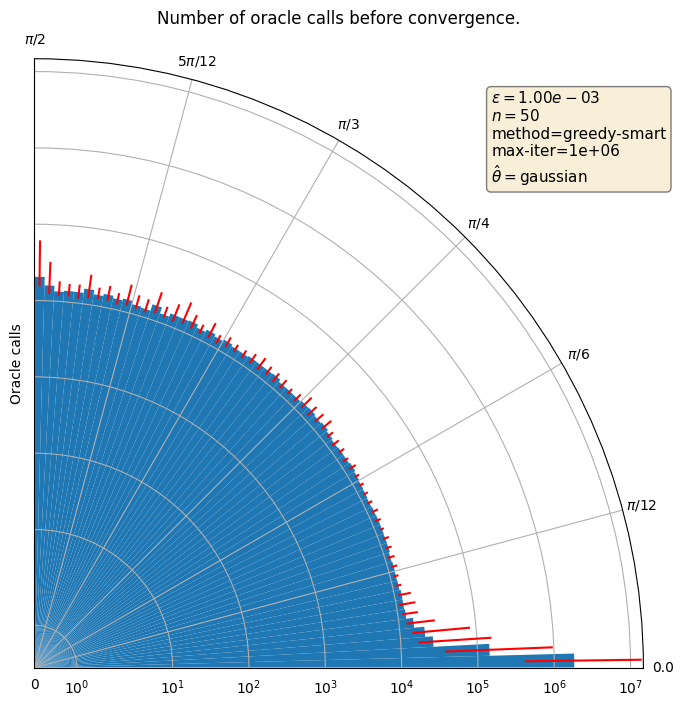
\includegraphics[width=\linewidth]{ExAE-converge-quarter-circle}
		\caption{Median number of oracle calls for SAE to converge to a precision of $\varepsilon = 10^{-3}$, with 25\% and 75\% quartiles shown. Each bar is a region of width $\pi / 120$ with the median number of oracle calls calculated from 50 values of true value $\theta_0$ selected uniformly at random. The prior for each iteration is taken to be $N(\tilde{\theta}_0, 1)$, where $\tilde{\theta}_0$ is sampled from a $N(\theta_0, 0.1)$ distribution and success probability $1 - \alpha$ with $\alpha = 0.01$.}
		\label{fig::ExAE-converge-quarter-circle}
	\end{subfigure}
	\hfill
	\begin{subfigure}{0.45\textwidth}
		\centering
		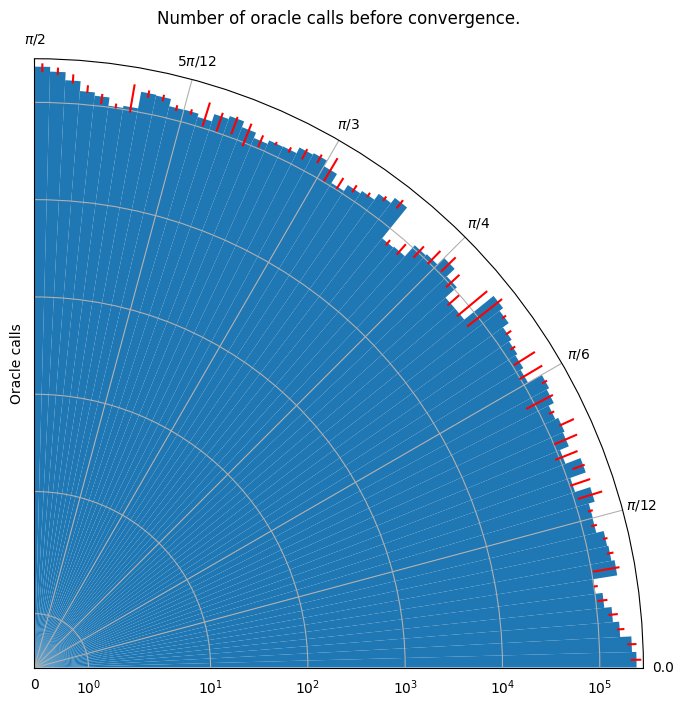
\includegraphics[width=\linewidth]{Iae-converge-quarter-circle}
		\caption{Median number of oracle calls for IAE to converge to a precision of $\varepsilon = 10^{-3}$, with 25\% and 75\% quartiles shown. Each bar is a region of width $\pi / 120$ with the median number of oracle calls calculated from 50 values of true value $\theta_0$ selected uniformly at random, and a success probability $1 - \alpha$ with $\alpha = 0.01$}
		\label{fig::Iae-converge-quarter-circle}
	\end{subfigure}
\end{figure}
\comment[id=cdv]{Misses a caption of the 'full' figure.}
\comment[id=cdv]{It's actually from 1000 values. I can change that either in the figure, or in the caption.}
\begin{center}
	\color{red}
	(The following is all conjecture as we don't have a comparison graph.) \\
As seen in Figure \ref{fig::ExAE-converge-on-theta1}, the set $\Theta_1$ performs poorly for all methods that take a statistical approach. This region contains points where the variance reduction factor approaches 0, with the extreme points where $\theta= 0, \pi$.
\end{center}

\begin{figure}[htbp]
	\centering
	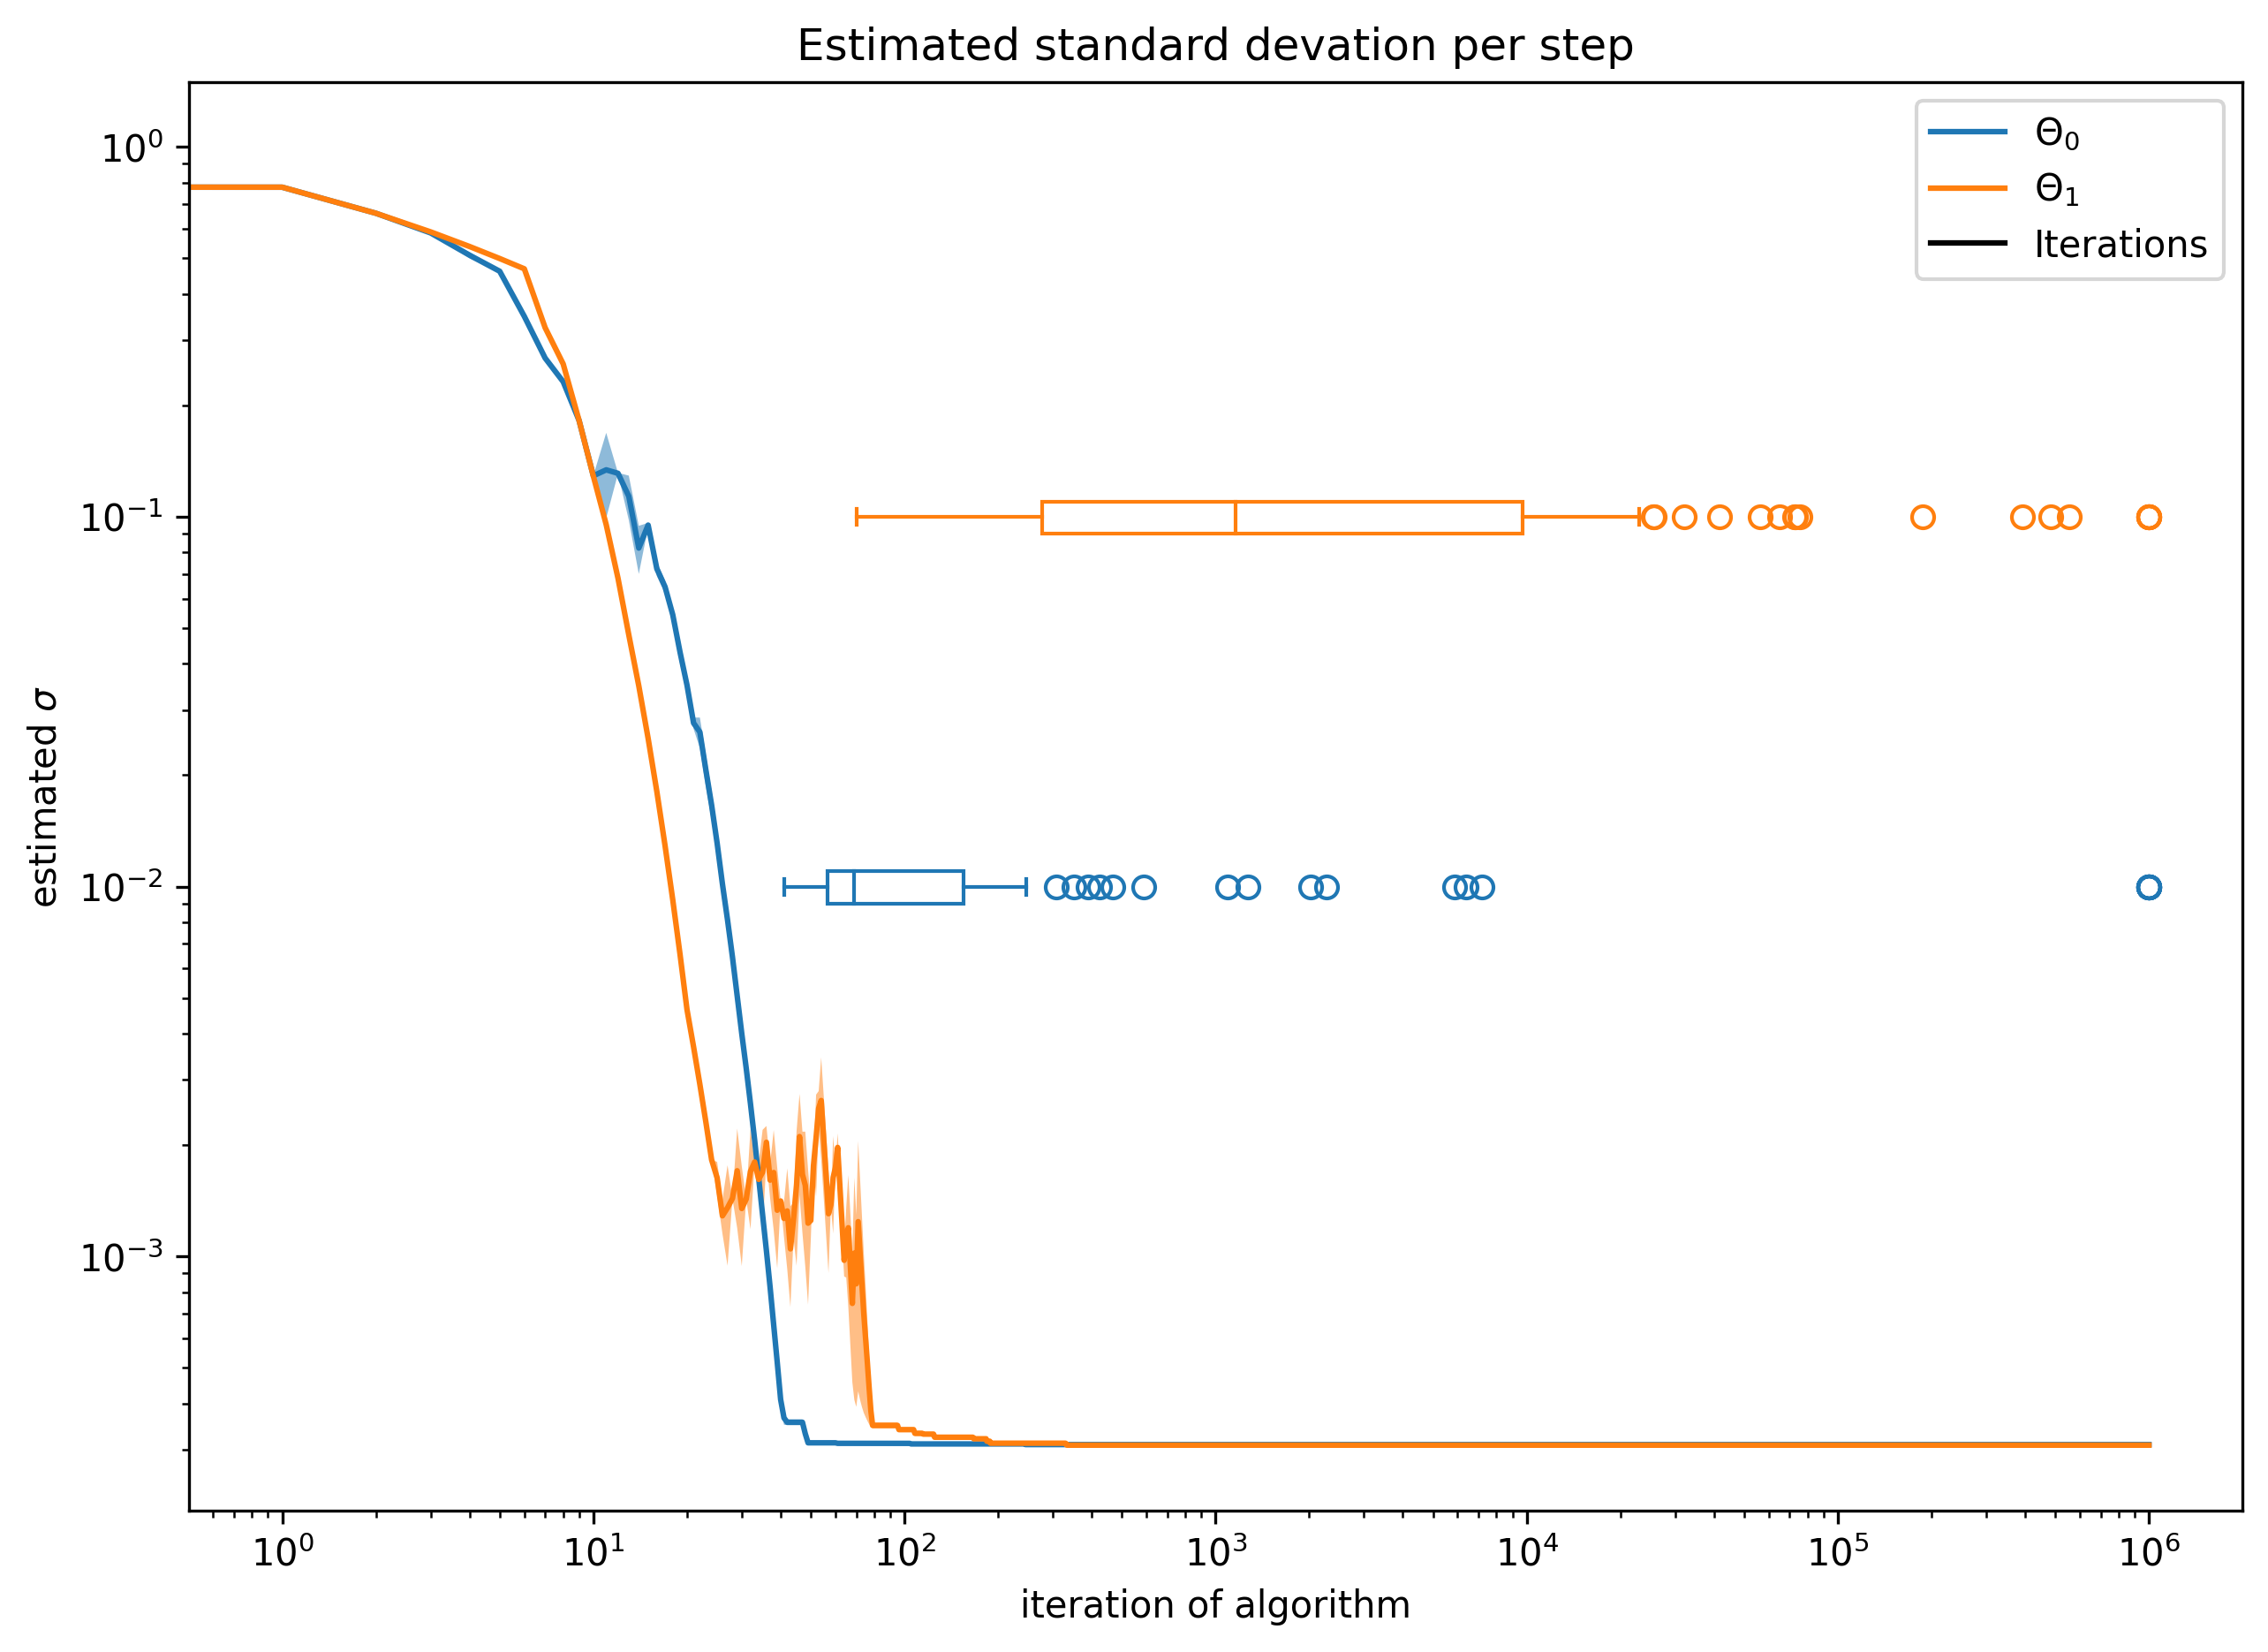
\includegraphics[scale=0.3]{ExAE-std-per-step}
	\caption{Median standard deviation for fixed error rate $\varepsilon = 10^{-3}$ against time step for $\theta_0 \in \Theta_0$ and $\theta_0 \in \Theta_1$. We sample $\theta_0$ from a uniform distribution of $x$ and $50$ samples for $\Theta_0$ and $ \Theta_1$ respectively. The prior for each iteration is taken to be $N(\theta_0, 1)$ and success probability $1 - \alpha$ with $\alpha = 0.01$. The box plots show the Q1, Q2 and Q3 algorithm termination times for the recorded runs.}
	\label{fig::ExAE-std-per-step}
\end{figure}

\begin{figure}[htbp]
	\centering
	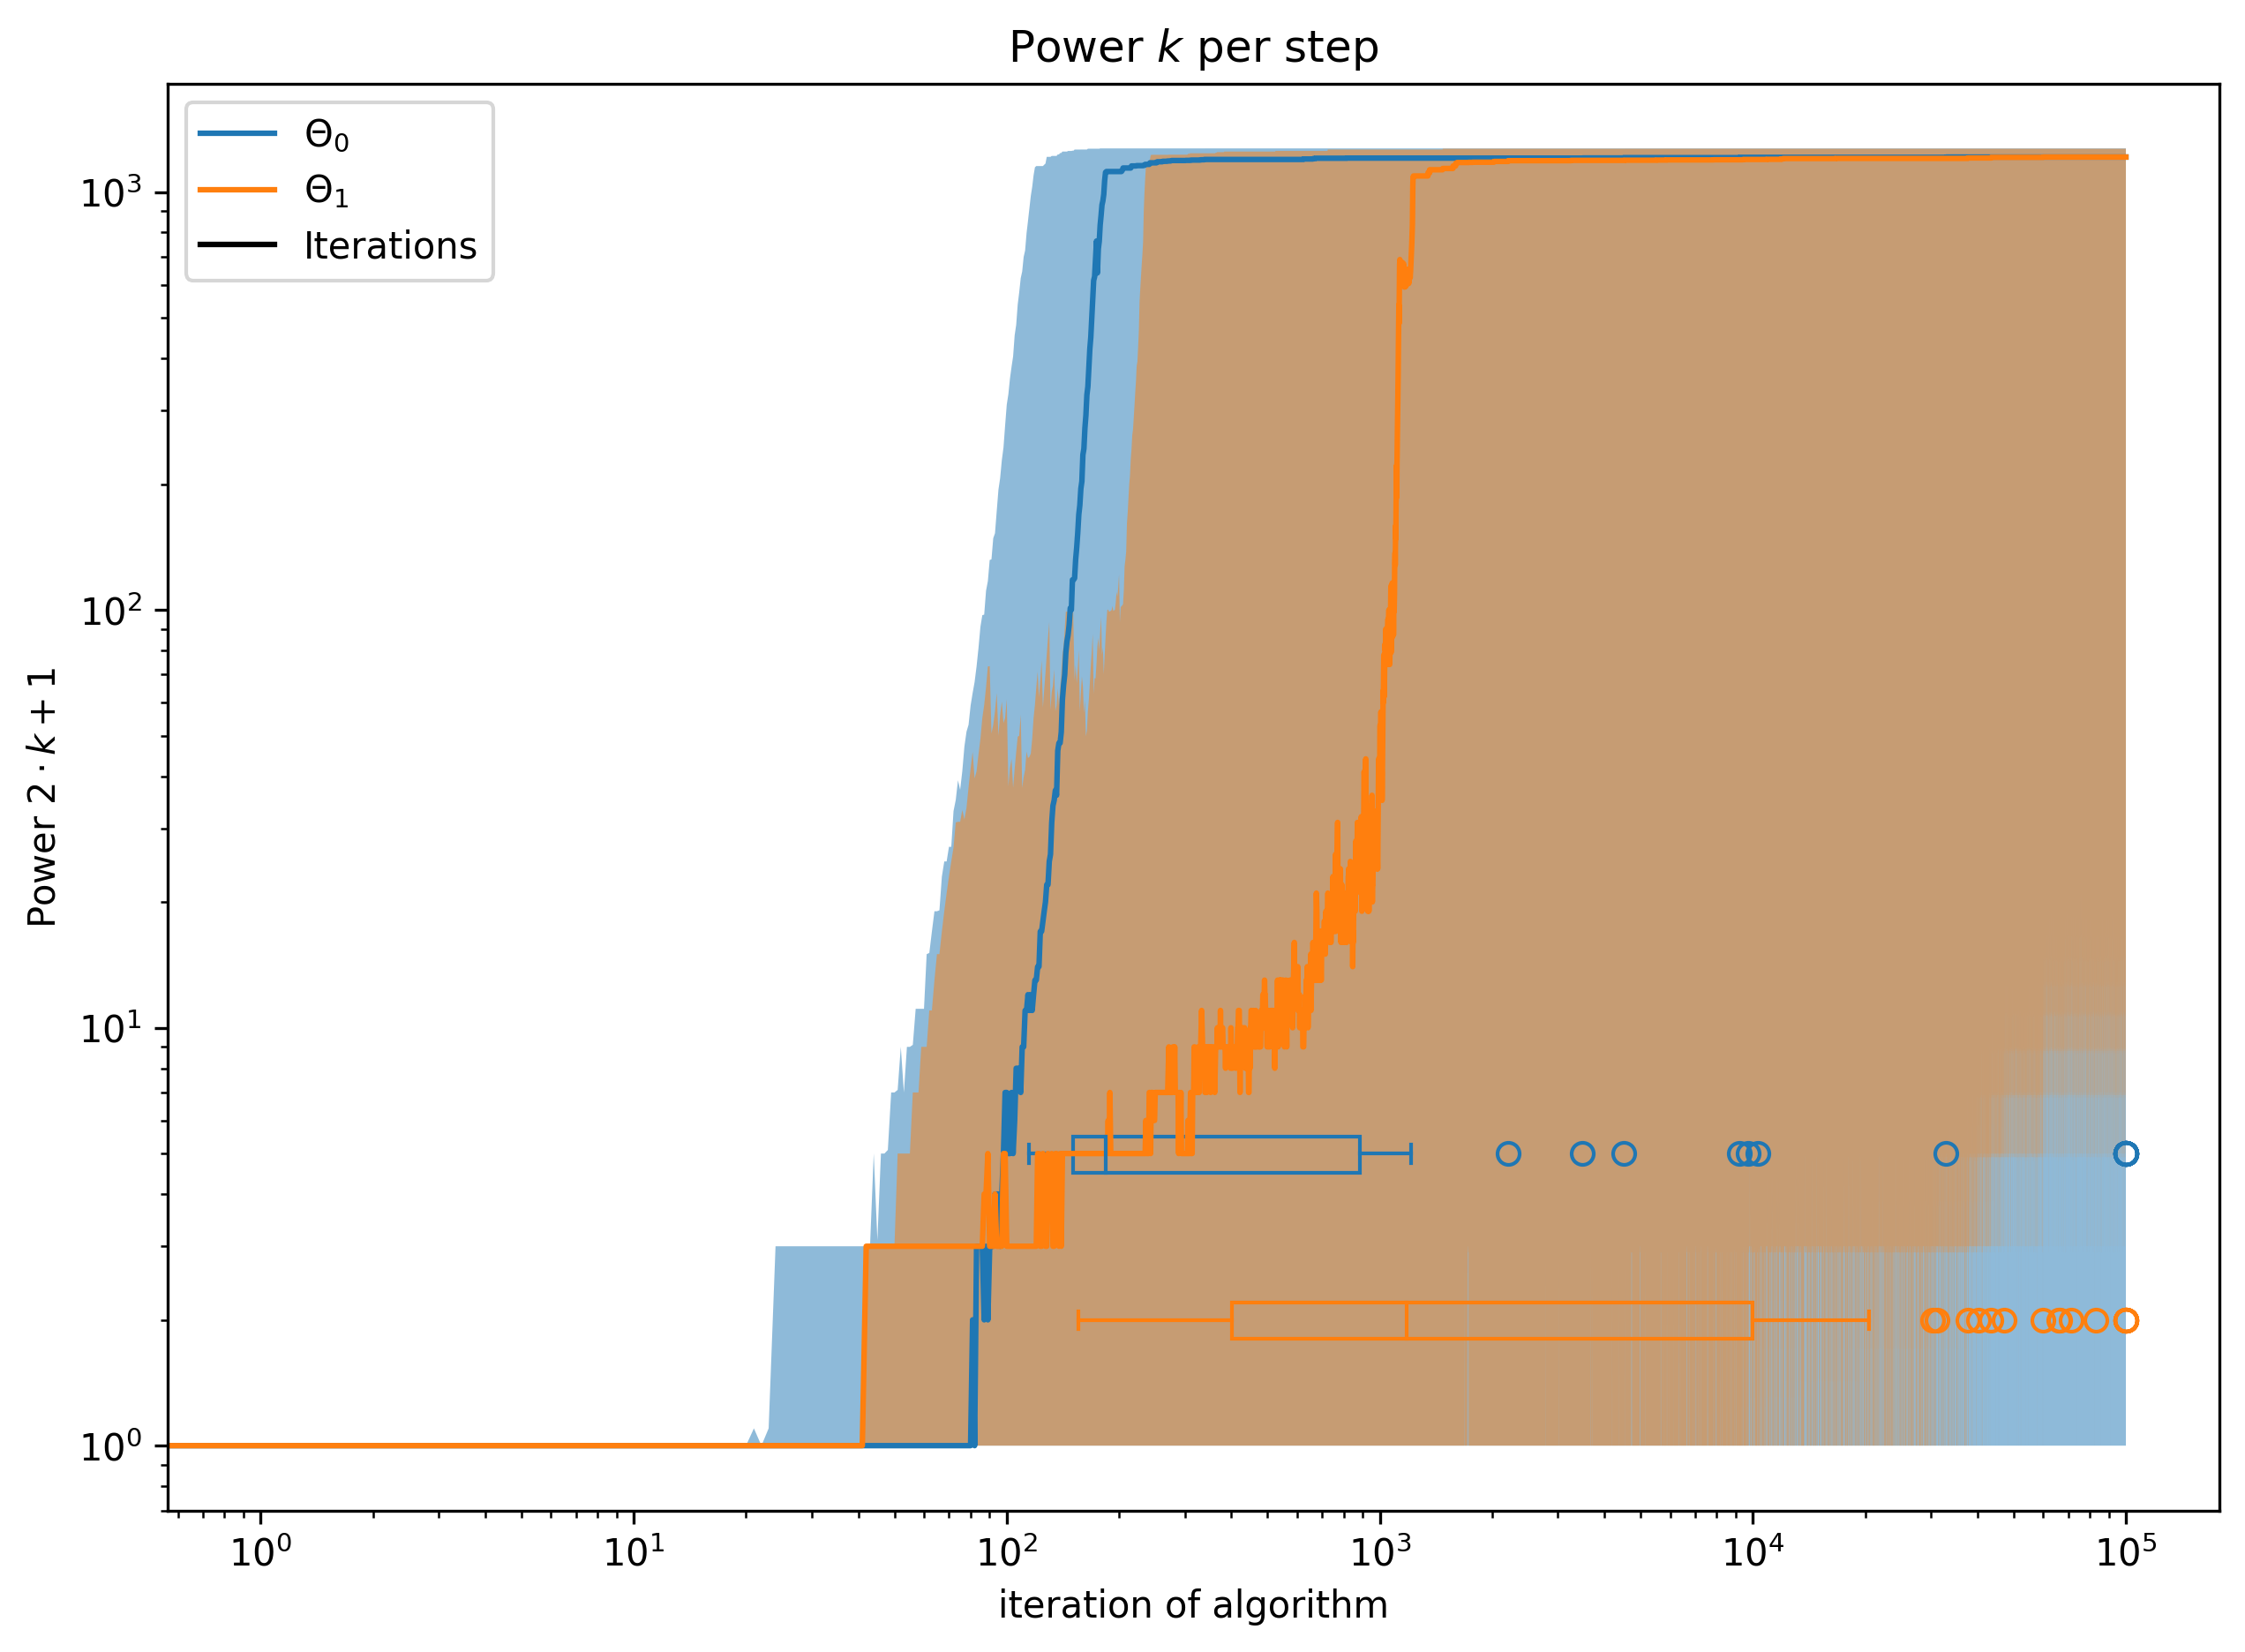
\includegraphics[scale=0.3]{ExAE-depth-per-step}
	\caption{Median depth for fixed error rate $\varepsilon = 10^{-3}$ against time step for $\theta_0 \in \Theta_0$ and $\theta_0 \in \Theta_1$. We sample $\theta_0$ from a uniform distribution of $x$ and $50$ samples for $\Theta_0$ and $ \Theta_1$ respectively. The prior for each iteration is taken to be $N(\theta_0, 1)$ and success probability $1 - \alpha$ with $\alpha = 0.01$. The box plots show the Q1, Q2 and Q3 algorithm termination times for the recorded runs.}
	\label{fig::ExAE-depth-per-step}
\end{figure}

From now on, we restrict to considering $\theta \in \Theta_0$.

A source of potential error in this algorithm is the normal approximation made at each step, which removes the theoretical guarantees of the Bernstein-von-Mises theorem. This can be seen in Figure \ref{fig::ExAE-actual-prec-vs-expected-prec}, where should expect $(1-\alpha)\%$ of the points to lie above the diagonal. As a mitigation technique, we post-process the measurement data using the MLE estimator, and recover some of the desired accuracy.

\begin{figure}[htbp]
	\centering
	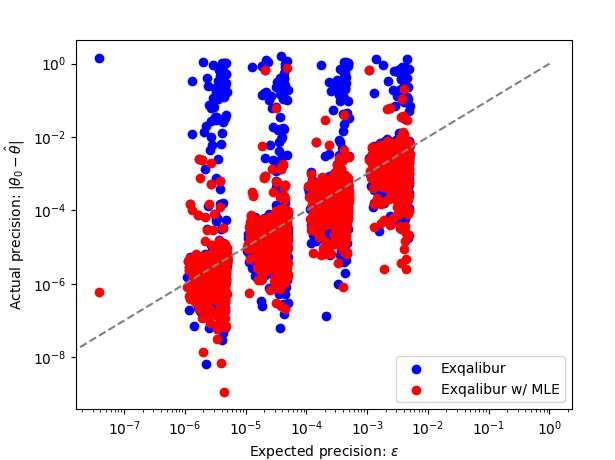
\includegraphics[scale=0.3]{ExAE-actual-prec-vs-expected-prec}
	\caption{Actual precision of the final estimate for SAE with and without MLE post-processing. We sample $\theta_0 \in \Theta_0$ from a uniform distribution of $x$ and $50$ for target precisions of $\varepsilon = 10^{-3}, 10^{-4}, \ldots, 10^{-7} $. The prior for each iteration is taken to be $N(\theta_0, 1)$ and success probability $1 - \alpha$ with $\alpha = 0.01$.}
	\label{fig::ExAE-actual-prec-vs-expected-prec}
\end{figure}

\begin{figure}[htbp]
	\centering
	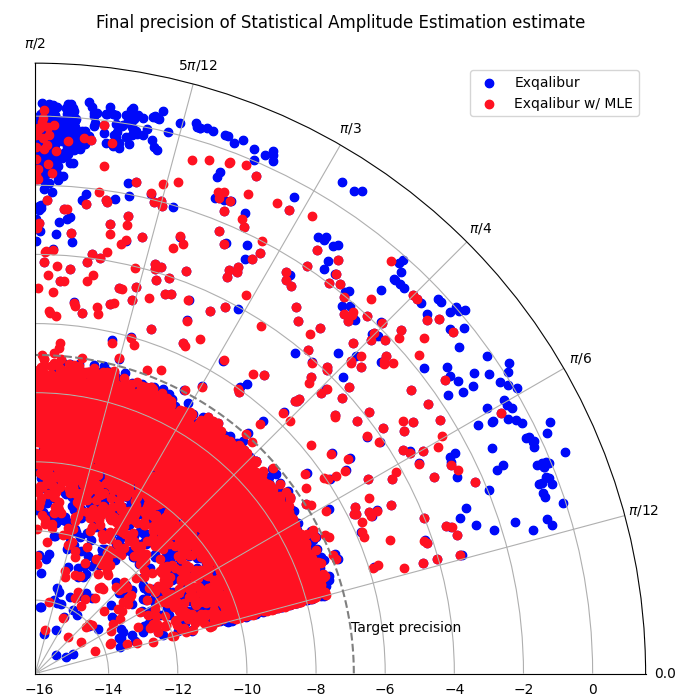
\includegraphics[scale=0.2]{ExAE-actual-prec-over-theta}
	\caption{Actual precision of the final estimate for SAE with and without MLE post-processing. We sample $\theta_0 \in \Theta_0$ from a uniform distribution of $x$ and $500$ for a target precision of $\varepsilon = 10^{-3}$. The prior for each iteration is taken to be $N(\theta_0, 1)$ and success probability $1 - \alpha$ with $\alpha = 0.01$.}
	\label{fig::ExAE-actual-prec-over-theta}
\end{figure}

We compare the performance of SAE to IAE and MLAE, and observe that in the noiseless case we achieve similar query to IAE. However, there still remain some points for which SAE fails to satisfactorily converge.

\begin{figure}[htbp]
	\centering
	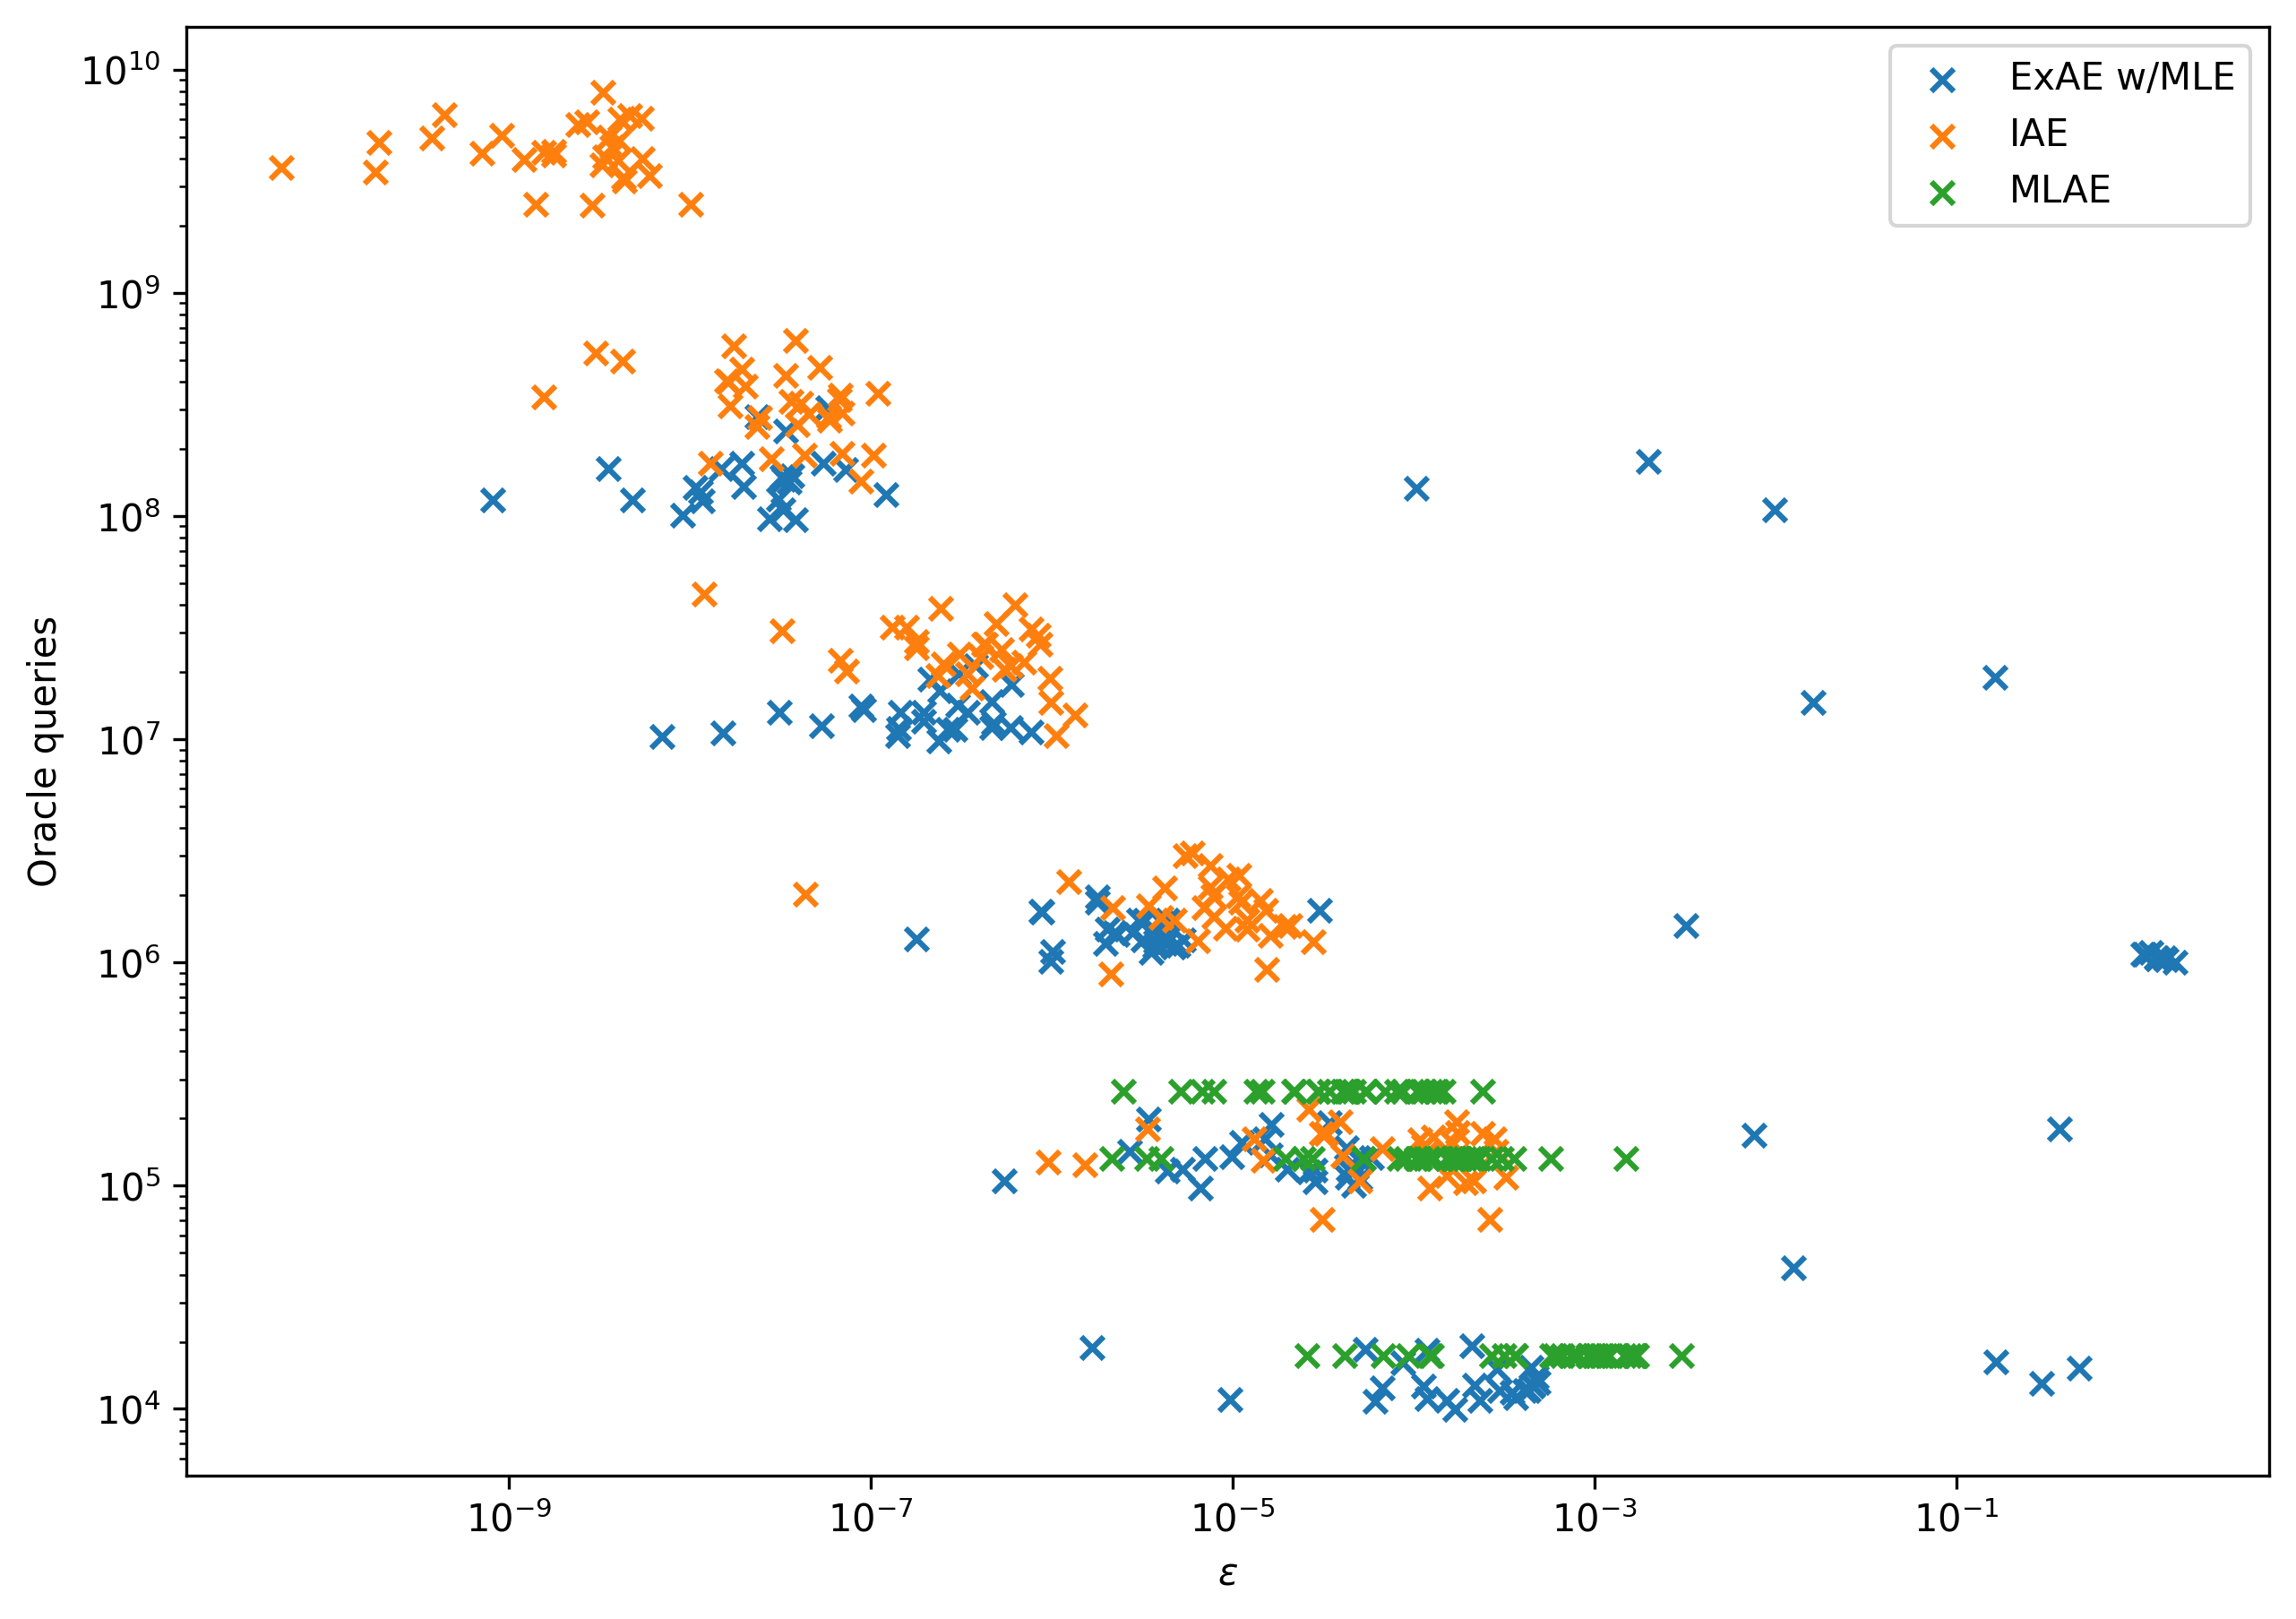
\includegraphics[scale=0.5]{query-comparison-noiseless}
	\caption{Actual precision versus total number of oracle queries used for IAE, MLAE and SAE. We target precisions of $\varepsilon = 10^{-3}, 10^{-4}, \ldots , 10^{-7}$, with each point a single value of $\theta_0 \in \Theta_0$ and take the final precision to be half the width of the confidence interval. We sample uniformly from $\Theta_0$ for 30 values of $\theta_0$. Each value of $\theta_0$ is evaluated for all algorithms and each target $\varepsilon$. The prior for each iteration is taken to be $N(\theta_0, 1)$ and success probability $1 - \alpha$ with $\alpha = 0.01$.}
	\label{fig::query-comparison-noiseless}
\end{figure}


\begin{figure}[htbp]
	\centering
	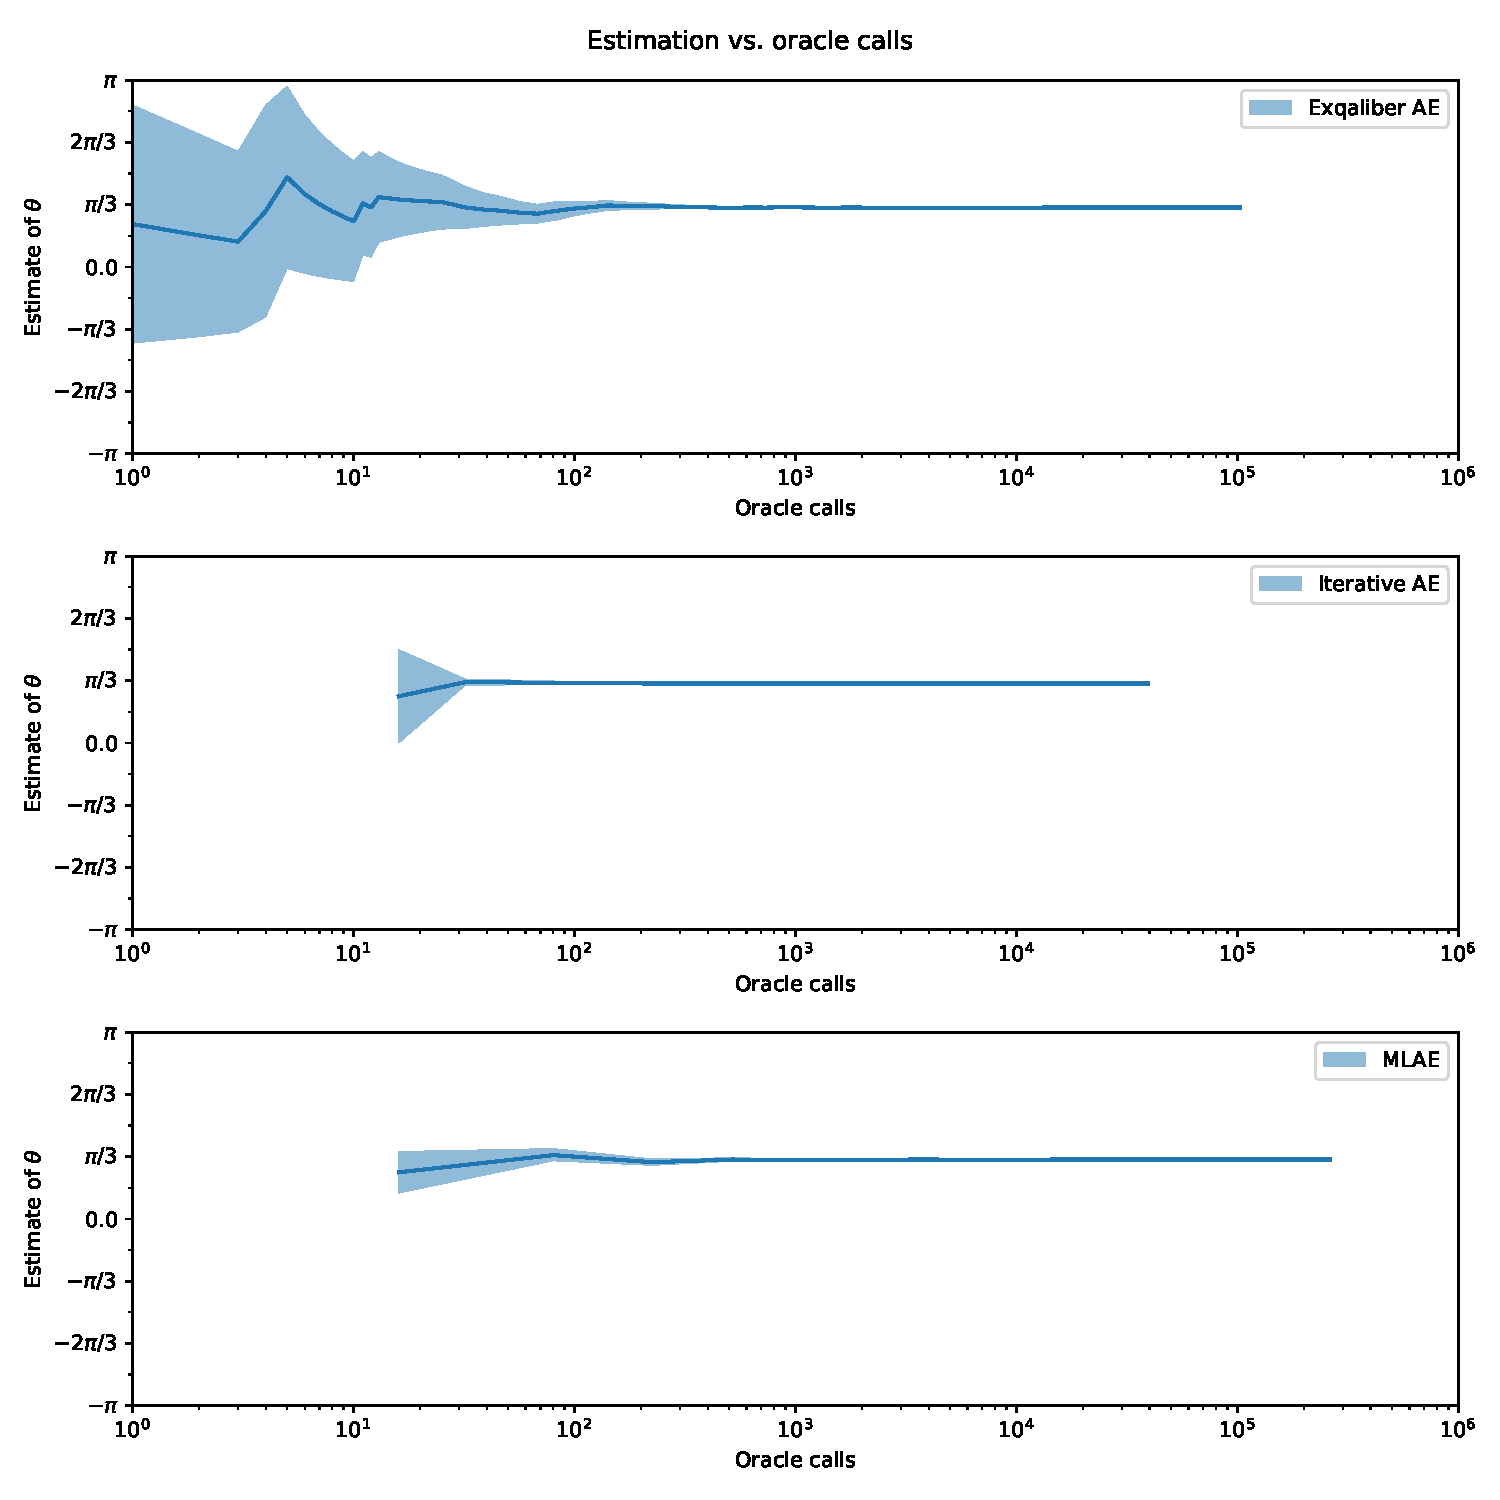
\includegraphics[scale=0.3]{compare-paths-oracle-calls}
	\caption{Confidence intervals for a single run of SAE, IAE and MLAE with $\theta_0 = 1$. The prior for SAE is taken to be $N(\pi/2, 1)$ and success probability $1 - \alpha$ with $\alpha = 0.01$. As IAE and MLAE use a fixed number of shots per step, the number of oracle calls does not start at 0.}
	\label{fig::compare-paths-oracle-calls}
\end{figure}

\subsubsection{Decohering Noise}
We explore the performance of our algorithm for a range of noise rates.

As shown in Figure \ref{fig::ExAE-noisy-max-depth}, the algorithm will not go beyond a depth of $\sim \frac{1}{\lambda}$.

\begin{figure}[htbp]
	\centering
	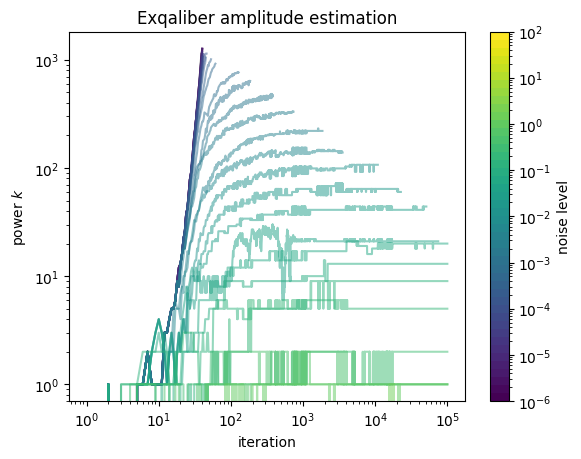
\includegraphics[scale=0.5]{ExAE-noisy-max-depth}
	\caption{Depth of SAE for $\theta_0 = 1$ at varying levels of decohering noise characterised by $\lambda = 10^0, 10^{-1}, \ldots 10^{-6}$. The prior for each iteration is taken to be $N(\pi /2, 1)$, we target $\varepsilon = 10^{-3}$ and success probability $1 - \alpha$ with $\alpha = 0.01$.}
	\label{fig::ExAE-noisy-max-depth}
\end{figure}

\begin{figure}[htbp]
	\centering
	\caption{Total number of oracle queries for SAE with decohering noise characterised by $\lambda = 10^{-1}, 10^{-2}, \ldots, 10^{-7}$. Each point is a single value of $\theta_0 \in \Theta_0$. We sample uniformly from $\Theta_0$ for 30 values of $\theta_0$. Each value of $\theta_0$ is evaluated for all decohering noise values and each target $\varepsilon$. The prior for each iteration is taken to be $N(\theta_0, 1)$ and success probability $1 - \alpha$ with $\alpha = 0.01$.}
	\label{fig::query-exae-noisy}
\end{figure}

\begin{itemize}
	\color{red}
	\item Concerned that error comparisons make no sense here. These algorithms have no capacity to cope with noise so obviously they're bad - but others e.g. Hitachi, QoPrime, Power-law AE do
\end{itemize}

\begin{figure}[htbp]
	\centering
	\caption{Final precision versus total number of oracle queries used for IAE, MLAE and SAE with decohering noise characterised by $\lambda = 10^{-3}$. We target precisions of $\varepsilon = 10^{-3}, 10^{-4}, \ldots , 10^{-7}$, with each point a single value of $\theta_0 \in \Theta_0$. We sample uniformly from $\Theta_0$ for 30 values of $\theta_0$. Each value of $\theta_0$ is evaluated for all algorithms and each target $\varepsilon$. The prior for each iteration is taken to be $N(\theta_0, 1)$ and success probability $1 - \alpha$ with $\alpha = 0.01$.}
	\label{fig::query-comparison-noisy}
\end{figure}

\newpage



%% This is probably explained earlier, but I need it for my argument, so I wrote it. In the final version, we probably need to refer to earlier in the text.
%In amplitude estimation, there is an operator $\mathcal{A}$ acting on $n+1$ qubits, such that $\mathcal{A} \ket{\psi}_{n+1} = \sqrt{a}\ket{\psi_1}_{n}\ket{1} + \sqrt{1-a}\ket{\psi_0}_n\ket{0}$,
%with $a\in [0,1]$ or, when defining $a=\sin^2{\theta_a}$ with $\theta_a \in [0, \pi]$,
%\begin{equation}
%	\mathcal{A}_{n+1} \ket{\psi} = \sin{\theta_a} \ket{\psi_1}_n \ket{1}
%	+ \cos{\theta_a}\ket{\psi_0}_n\ket{0}.
%\end{equation}
%The goal is to find $\theta_a$.
%
%One can create an operator $\mathcal{Q} = \mathcal{A} \mathcal{S}_0 \mathcal{A}^{\dagger}\mathcal{S}_{\psi_0}$ with $\mathcal{S}_{\psi_0} = \mathbb{I} - 2\ket{\psi_0}_n\bra{\psi_0}_n\otimes\ket{0}\bra{0}$ and $\mathcal{S}_0 = \mathbb{I} - 2\ket{0}_{n+1}\bra{0}_{n+1}$. % TODO reference
%% TODO choose definition of 'oracle queries'. In the iterative AE paper, they "denote applications of Q as quantum samples or oracle queries."
%Now by applying $\mathcal{Q}$ for $k$ times (and thereby applying $\mathcal{A}$ a total of $(2k+1)$ times), the probability of measuring the $\ket{1}$ state follows a Bernoulli distribution with $p$ equal to
%\begin{equation}
%	p = \frac{1}{2}(1-\cos{((2k+1)\theta_a)}).
%	\label{eq:bernoulli-p}
%\end{equation}
%Using this equation, one can test different amplitude estimation analytically, by sampling from the Bernoulli distribution directly. We call this direct analytical sampling.
%
%We experimented with our novel amplitude estimation routine. There are two relevant measures for amplitude estimation.
%These are the time to solution (and its scaling) and the quality of the solution, i.e., the error $\epsilon$.
%To measure these, we simulate experiments using direct analytical sampling.
%
%
%As our algorithm uses dynamical updates, depending on the true $\theta$, %TODO: make this consistent throughout the article. Maybe theta hat?
%anomalies can rise for values around integer fractions of $\pi$.

\section{Discussion} \label{sec::discussion}
TO BE ADDED
\begin{itemize}
	\item Summary what we have done
	\item The potential incorporating for error mitigation and error correction
	\item Wider noise models
	\item How can we further bring down the requirements to accelerate?
	\item How can it be used for QPE style
\end{itemize}


%This is for internal discussions not external release
%Topics to include here include:
%\begin{itemize}
%	\item Directions for future including reinforcement learning
%	\item Superconducting and trapped ion thought experiment
%	\item Discussion about general dynamic programming approach for considering error mitigation and correction
%	\item Connection to QPE and applicability of thinking to that setting (maybe include small section on the more complicated statistical challenge of general state)
%	\item Circular distributions and what we know about them (probably subsection of this section or algorithm)
%\end{itemize}

\newpage


\bibliographystyle{quantum}
\bibliography{exqaliber-phase1-bibliography.bib}

\appendix

\section{Posterior statistics}
In this appendix, we calculate all statistics of interest for the posterior distribution.
\subsection{Noiseless}
\label{app::noiseless}
In the noiseless case, we consider a prior distribution $\pi(\theta) \sim N(\mu, \sigma^2)$ and our sampling distribution $X \sim \text{Ber}(\frac{1}{2} (1 - \cos((4d+2) \theta))$. First, let us calculate all the moments of the posterior distribution, given the measurement:
\[
	\mathbb{E}\left[ \theta^{m} | X = x \right] = \frac{\int_{- \infty}^{\infty} \theta^{m} \left( 1 + \left( -1 \right) ^{x} \cos\left( 2\left( 2d + 1 \right) \theta \right)  \right) e^{-\frac{1}{2 \sigma^2} \left( \theta - \mu \right) ^2} \text{d}\theta}{\int_{- \infty}^{\infty} \left( 1 + \left( -1 \right) ^{x} \cos\left( 2\left( 2d + 1 \right) \theta \right)  \right) e^{-\frac{1}{2 \sigma^2} \left( \theta - \mu \right) ^2} \text{d}\theta}
.\]
Thus, the integrals of interest take the form.
\[
I_m(\theta) = \int_{- \infty}^{\infty} \theta^{m} \left( 1 + \left( -1 \right) ^{x} \cos\left( 2 \left( 2 d + 1 \right) \theta \right)  \right) e^{- \frac{1}{2 \sigma^2} \left( \theta - \mu \right) ^2}\text{d}\theta
.\]
For the following, we're going to define the Fourier transform $\hat{f}\left( \omega \right) $ to be given by
\[
	\hat{f}\left( \omega \right) = \int_{- \infty}^{\infty} f(x) e^{ - i \omega x}\text{d}x = \mathcal{F}\left\{ f(x) \right\} ,
\]
for some function $f(x)$. We also recall the following facts about the Fourier transform:
\begin{align}
&	\mathcal{F}\left\{ f(x-a) \right\} \mapsto e^{- i a \omega}\hat{f}(\omega)\label{eqn::fourier-trans}	\\
&	\mathcal{F}\left\{ f(ax) \right\}   \mapsto \frac{1}{|a|}\hat{f}(\frac{\omega}{a}) \label{eqn::fourier-mult} \\
&	\mathcal{F}\left\{ x^{n}f(x) \right\}  \mapsto i^{n} \frac{\text{d}^{n} \hat{f}(\omega)}{\text{d}\omega^{n}} \label{eqn::fourier-power} \\
&	\mathcal{F} \left\{ e^{- x^2} \right\}  = \sqrt{\pi} e^{- \frac{\omega^2}{4}}. \label{eqn::fourier-gauss}
\end{align}
We can now rewrite $I_m(\theta)$ to be in a suitable Fourier form,
\[
	I_m(\theta) = \sqrt{2 \pi \sigma^2} \mathbb{E}_{\pi(\theta)}\left[ \theta^{m} \right]  + \frac{ \left( -1 \right)^{x} }{2}\int_{- \infty}^{\infty} \theta^{m} \left( e^{2(2d + 1)i \theta} + e^{ - 2(2d+1)i\theta}\right) e^{- \frac{1}{2 \sigma^2} \left( \theta - \mu \right) ^2}\text{d}\theta
.\]
Consider
\begin{align*}
& \int_{-\infty}^{\infty}e^{-\frac{\theta^2}{2 \sigma^2}}e^{- i \omega \theta} \text{d}\theta = \sqrt{2 \pi \sigma^2} e^{-\frac{\sigma^2 \omega^2}{2}}, & \text{by } (\ref{eqn::fourier-gauss}) \text{ and } (\ref{eqn::fourier-power})\text{, taking }a = \frac{1}{\sqrt{2 \sigma^2} }, \\
&	\int_{- \infty}^{\infty} e^{- \frac{1}{2 \sigma ^2}\left( \theta-\mu \right)^2  } e^{ -i \omega \theta}\text{d} \theta = \sqrt{2 \pi \sigma^2}   e^{- i \mu\omega}e^{- \frac{\sigma^2 \omega^2}{2}}, & \text{by } (\ref{eqn::fourier-trans}), \text{ taking } a = \mu, \\
& \int_{- \infty}^{\infty} \theta^{m}e^{-\frac{1}{2 \sigma^2}\left( \theta - \mu \right)^2 }e^{ - i \omega \theta}\text{d}\theta = i^{m}\frac{\text{d}^{m}}{\text{d}\omega^{m}}\left( \sqrt{2\pi \sigma^2}  e^{- i \mu \omega} e^{- \frac{\sigma^2 \omega^2}{2}} \right), & \text{by } (\ref{eqn::fourier-power}), \\
& \int_{- \infty}^{\infty} \theta^{m} e^{-\frac{1}{2 \sigma^2}\left( \theta - \mu \right)^2 } e^{i \omega \theta}\text{d}\theta = (-i)^{m}\frac{\text{d}^{m}}{\text{d}\omega^{m}}\left( \sqrt{2 \pi \sigma^2}  e^{ i \mu \omega} e^{- \frac{\sigma^2 \omega^2}{2}} \right), & \text{by } \omega \mapsto - \omega. \\
\end{align*}
From which we conclude
\[
	I_m(\theta) = \sqrt{2 \pi \sigma^2} \left[ \mathbb{E}_{\pi(\theta)}\left[ \theta^{m} \right] + \left( -1 \right)^{x}   \left. \frac{\text{d}^{m}}{\text{d}\omega^{m}}\right\vert_{\omega = 2(2d+1)}\left( \frac{e^{i \mu \omega} + \left( -1 \right)^{m}e^{- i \mu \omega}}{2 i^{m}}  e^{ - \frac{\sigma^2 \omega^2}{2}} \right)   \right]
.\]
In particular,
\begin{align*}
	I_0\left( \theta \right) &= \sqrt{2 \pi \sigma^2} \left( 1 + \left( -1 \right) ^{x}e^{- 2 \left( 2d+1 \right)^2 \sigma^2} \cos\left( 2\left( 2d+1 \right) \mu \right)  \right] \\
	I_1(\theta) &= \sqrt{2 \pi \sigma^2}\left[ \mu + (-1)^{x} \left. \frac{\text{d}}{\text{d} \omega}  \right\vert_{\omega =2(2d+1) } \left( \sin \left( \mu \omega \right)  e^{ - \frac{\sigma^2 \omega^2}{2}} \right)  \right]  \\
		    &= \sqrt{2\pi \sigma^2} \left[ \mu + \left( -1 \right) ^{x}e^{ - 2\left( 2d+1 \right) ^2 \sigma^2} \left( \mu \cos\left( 2\left( 2d+1 \right) \mu \right)  - 2\left( 2d+1 \right) \sigma^2 \sin \left( 2\left( 2d+1 \right) \mu \right)  \right) \right] \\
		I_2\left( \theta \right) & = \sqrt{2 \pi \sigma^2} \left[ \sigma^2 + \mu^2 - \left( -1 \right) ^{x} \left. \frac{\text{d}^2}{\text{d}\omega^2} \right\vert_{\omega = 2\left( 2d+1 \right) }\left( \cos\left( \mu \omega \right) e^{- \frac{\sigma^2 \omega^2}{2}} \right)  \right]\\
					 &= \sqrt{2 \pi\sigma^2} \left[ \sigma^2 + \mu^2 + \left( -1 \right) ^{x} e^{- 2\left( 2d+1 \right) ^2 \sigma^2}\left( \left( \mu^2 + \sigma^2- 4\left( 2d+1 \right) ^2\sigma^{4} \right) \cos\left( 2\left( 2d+1 \right) \mu \right) \right. \right. \\
					 & \hspace{225pt} \left. \left.   - 4\left( 2d+1 \right) \mu\sigma^2 \sin\left( 2\left( 2d+1 \right) \mu \right)  \right) \right]
\end{align*}

Hence
\begin{align}
	\mathbb{E}\left[ \theta | X = x \right] & = \mu - \left( -1 \right) ^{x}e^{ - 2\left( 2d+1 \right) ^2 \sigma^2} \frac{2 \left( 2d+1 \right) \sigma^2 \sin \left( 2\left( 2d+1 \right) \mu \right) 	}{1 + \left( -1 \right) ^{x}e^{ - 2 \left( 2d+1 \right) ^2 \sigma^2} \cos\left( 2\left( 2d+1 \right) \mu \right) } \\
	\text{Var}\left( \theta | X= x \right) &= \sigma^2\left( 1 - \left( -1 \right) ^{x}4\left( 2d+1 \right) ^2 \sigma^2 e^{ - 2 \left( 2d+1 \right) ^2 \sigma^2} \frac{\cos\left( 2\left( 2d+1 \right) \mu \right)  + \left( -1 \right) ^{x}e^{ - 2 \left( 2d+1 \right) ^2 \sigma^2}}{\left( 1 + \left( -1 \right) ^{x} e^{- 2 \left( 2d+1 \right) ^2 \sigma^2} \cos \left( 2 \left( 2d+1 \right) \mu \right)  \right) ^2} \right) \\
					       &=\sigma^2 \left( 1 - \sigma^2 \mathcal{V}_x  \right),
\end{align}
where we define
\[
	\mathcal{V}_x = \left( -1 \right) ^{x} 4\left( 2d+1 \right) ^2 e^{ - 2 \left( 2d+1 \right) ^2 \sigma^2} \frac{\cos\left( 2\left( 2d+1 \right) \mu \right) + \left( -1 \right) ^{x} e^{ - 2 \left( 2d+1 \right) ^2 \sigma^2}}{\left( 1 + \left( -1 \right) ^{x} e^{ - 2 \left( 2d+1 \right) ^2 \sigma^2} \cos\left( 2 \left( 2d+1 \right) \mu \right)  \right) ^2}
.\]
If we note that $\mathbb{P}\left( X = x \right) = \frac{I_0\left( \theta, x \right)}{2\sqrt{2 \pi \sigma^2} } $, then we recover $\mathbb{E}[\theta] = \mu$. Similarly, we obtain
\[
	\text{Var}\left( \theta \right) = \sigma^2\left( 1 - \sigma^2 \mathcal{V} \right)
,\]
where
\begin{align*}
	\mathcal{V} &= \mathbb{P}\left( X = 0 \right) \mathcal{V}_0 + \mathbb{P}\left( X = 1 \right) \mathcal{V}_1 \\
		    &= \frac{ 2\left( 2d+1 \right) ^2 e^{ - 2 \left( 2d+1 \right) ^2 \sigma^2}}{1 - e^{ - 4 \left( 2d+1 \right) ^2 \sigma^2} \cos\left( 2\left( 2d+1 \right) \mu \right) } \times \\
		    &	\qquad \left\{   \left( \cos\left( 2 \left( 2d+1 \right) \mu \right) + e^{ - 2 \left( 2d+1 \right) ^2 \sigma^2} \right) \left( 1 - e^{ - 2\left( 2d+1 \right) ^2 \sigma^2}\cos\left( 2\left( 2d+1 \right) \mu \right)  \right) \right. \\
		    & \qquad \left. - \left( \cos\left( 2\left( 2d+1 \right) \mu \right) -e^{- 2 \left( 2d+1 \right) ^2 \sigma^2} \right) \left( 1 + e^{ - 2 \left( 2d+1 \right) ^2 \sigma^2}\cos\left( 2\left( 2d+1 \right) \mu \right)  \right)  \right\} \\
		    &= \frac{4\left( 2d+1 \right) ^2 e^{ - 4\left( 2d+1 \right) ^2 \sigma^2} \sin^2 \left( 2\left( 2d+1 \right) \mu \right) }{1 - e^{ - 4\left( 2d+1 \right) ^2 \sigma^2} \cos^2 \left(  2 \left( 2d+1 \right) \mu \right) }
\end{align*}


\subsection{Noisy} \label{app:noise}
In the noisy case, we consider the use of a depolarising quantum channel $\Phi\left( \cdot \right) $ with depolarising probability $p$. For any quantum state $\rho$, we have
\[
\Phi\left( \rho \right) = \left( 1- p \right) \rho + p\frac{\rho}{2^{n}}I, \quad 0 \le p \le 1 + \frac{1}{2^{2n} - 1}
,\]
where $I$ is the density matrix corresponding to the maximally mixed state on $2^{n}$ qubits. As the most error-prone part of the quantum circuit is the use of the state preparation routine $\mathcal{A}$, we consider only the probability that the state is properly prepared after each application of $\mathcal{A}$
\[
\prod_i \left( 1 - p_i \right) \approx e^{- \lambda}, \quad \text{for } \lambda = \sum_i p_i,
\]
for $\lambda \sim 1$ by a Poisson approximation, where  $p_i$ is the depolarising probability for each gate $A_i$ applied. Hence, we approximate the probability that we generate $\mathcal{U}^{d} \mathcal{A} \ket{0}^{\otimes n}$ as $e^{-\left( 2d+1 \right) \lambda}$ and generate the maximally mixed state otherwise. Therefore,
\[
	\mathbb{P}\left( X = x| \, \theta, \lambda \right) = \frac{1}{2}\left( 1 - \left( -1 \right) ^{x} e^{ - \left( 2d+1 \right) \lambda} \cos\left( 2\left( 2d+1 \right) \theta \right)   \right)
.\]
We note that this exponentially suppress the signal we get from our angle $\theta$

\section{Multiplicative bias of the standard variance estimator} \label{app::logvar}

\section{Multiplicative convergence of RAE} \label{app::decrease}

\end{document}
